\documentclass[11pt]{article}
\usepackage[margin=1in]{geometry}
% T1 fontenc omitted: cm-super is not installed here; OT1 Computer Modern Type 1 fonts are used
\usepackage[utf8]{inputenc}
% lmodern omitted: not needed with the standard fonts
\usepackage[expansion=false]{microtype}
\usepackage{booktabs}
\usepackage{array}
\usepackage{multirow}
\usepackage{amsmath}
\usepackage{graphicx}
\usepackage{xcolor}
\usepackage[hidelinks]{hyperref}
\usepackage[numbers,sort&compress]{natbib}
\usepackage{caption}
\captionsetup{font=small,labelfont=bf}

\newcommand{\rep}[1]{\texttt{#1}}
\newcommand{\ci}[2]{[\ensuremath{#1},\,\ensuremath{#2}]}  % math minus signs in intervals
\setlength{\emergencystretch}{2em}  % intervals do not break; let lines stretch instead

\title{A few vectors for a mixed folder:\\a pre-registered measurement of pooled directory embeddings}
\author{Ali Basheer\\Craftpine Inc., Toronto\\\texttt{ali@basheerali.com}}
\date{October 2026}

\begin{document}
\maketitle

\begin{abstract}
A folder's metadata is read before its files and holds a few kilobytes. A vector stored there can route a query without opening the folder, and the cheapest is the mean of its files' embeddings. We ask when the mean is enough and what to store when it is not. Under our main vision-language embedder, the mean does at least as well as a few representatives on GitHub directories that do not mix media, about 95 percent of those eligible. Representatives for mixed folders only are level with the mean over all directories (both post hoc). Where a folder mixes images and texts, the mean loses its minority modality. On Zenodo record folders a held-out minority file finds its folder 0.16 to 0.25 recall@5 less often with the mean than with a few per-modality representatives under two vision-language embedders, and 0.35 to 0.50 less often under two CLIP-family dual towers. There, four representatives per label are not inferior to searching every file, at a 0.02 margin, over all queries and in every cell under all four encoders (post hoc). On queries that a language model wrote as a simulated searcher, the loss under the main embedder is 0.14 (interval 0.02 to 0.28) for pictures in text-heavy folders and 0.42 (0.28 to 0.56) for documents in image-heavy ones. At three per label every folder's representatives fit in 8 KiB at a further cost of at most 0.012 in any cell. In 2 KiB a per-kind sample of the folder's files keeps the minority files the mean loses, and on ext4 a summary of 2,048 or 4,000 bytes costs 1.2 blocks per cold directory read. With every creator weighted equally the main embedder's file-query loss is 0.13 and 0.14, and 0.06 and 0.12 on queries whose names do not give the folder away. Every hypothesis was fixed in a brief before its test. Five briefs are timestamped externally, the rest dated by the working repository's history. Code, manifests and briefs are released.
\end{abstract}

\section{Introduction}

A file system reaches a folder before it reaches the folder's files. The folder's own metadata can be read without listing or opening anything inside it, but it holds little. An extended attribute, a named value attached to a file or a directory, holds at most 64 KiB on Linux, and Microsoft's abstract file system model for the SMB protocols allows one file's attributes just under 64 KB in total \citep{linux2026xattr,microsoft2025msfsa}. Common configurations keep them smaller. On ext4 a file's attributes normally have to fit in its inode and one block of at most 4,096 bytes, and APFS stores a value inside the file-system record up to 3,804 bytes \citep{linux2026xattr,e2fsprogs2025ext4,apple2020apfs}. A vector kept in such a field can be read before a search decides whether to open the folder, and it has to fit in a fixed number of bytes. This is the setting we have in mind. File-level search needs the vector of every file, which a search in this setting has not yet read, so we treat it as the reference and ask how much of it a few kilobytes on the folder keep.

Folders are becoming units of retrieval again. Retrieval-augmented generation routes a query to a source before it searches inside it, and one router takes the centroid of each source's document embeddings as an input \citep{dhasade2026ragroute}. Routers over expert embedding models keep centroid pilot embeddings \citep{lee2025routerretriever}. A context database for agents organises resources, memories and skills as a directory tree whose directories carry a short abstract used for vector retrieval \citep{openviking2026docs}. Vector databases are adding directory-scoped queries \citep{wang2026directoryaware}, and semantic file systems, an idea from 1991 \citep{gifford1991sfs}, now have embedding-backed descendants \citep{perone2025vectorvfs}. The cheapest representation of a container in an embedding space is the mean of its members' vectors. It is the dense counterpart of the single bag of words by which early federated search summarised a collection \citep{callan1995cori,shokouhi2011federated}.

Containers of files mix media. A record of a field study holds photographs, a scanned permit, a spreadsheet of readings and a README. Several embedders put such files in one space \citep{gunther2025jinav4,koukounas2024jinaclipv2,zhang2025gme,nussbaum2024nomicvision}. In contrastive models, image and text embeddings occupy offset regions of that space \citep{liang2022mindgap}, and in mixed-modality retrieval the offset biases ranking toward the query's own modality \citep{li2025grclip}. The authors of the vision-language embedder used for most of this study report the gap dramatically reduced \citep{gunther2025jinav4}, and it still shows one on our files (Section~\ref{sec:mechanism}). That work studies single items. That one mean misrepresents a group made of two clusters is expected, and textbook material for classifiers \citep{manning2008iir}. To our knowledge, nobody has measured how much a pooled vector loses on real mixed-media folders, or what a folder's few kilobytes can keep instead.

We measure it here, and ask when the mean is enough. Most answers below rest on hypotheses whose criteria were fixed before they were tested, and the analyses that a round of review prompted on draws already read are marked post hoc. We answer on three disjoint draws of real Zenodo record folders that followed a pilot draw, on two draws of directories of public GitHub repositories and on whole repository trees. For folders of the last Zenodo draw, a language model also wrote queries as a simulated searcher. Four encoders from three vendors take part, two vision-language embedders and two CLIP-family dual towers. Figure~\ref{fig:setup} sketches the setup.

\begin{figure}[t]
\centering
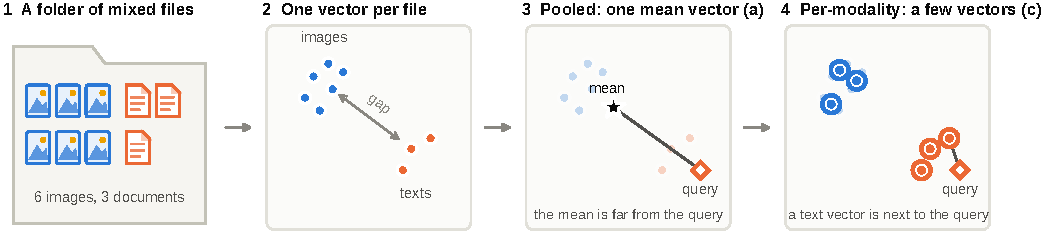
\includegraphics[width=\textwidth]{figures/fig_setup.pdf}
\caption{How a folder is represented and scored (a schematic, not data). (1) A folder holds images and documents. (2) Each file becomes a vector in one shared space, and the images and the texts land in two regions. (3) The pooled representation \rep{a} keeps one vector, the mean of the folder's files, which sits between the two regions. (4) The per-modality representation \rep{c} keeps a few $k$-means vectors for each modality. A folder's score for a query is the best cosine between the query and the folder's vectors. A text query held out from this folder is far from the mean and next to one of the folder's text vectors.}
\label{fig:setup}
\end{figure}

\begin{enumerate}
\item \textbf{When is the mean enough?} Mixed directories are 4 to 5 percent of eligible GitHub directories, and on the others the mean does at least as well as a few representatives under the first of the two vision-language embedders (post hoc). A file system can tell the mixed ones by file type. Keeping representatives only for folders that hold an image and another file keeps most of the minority gain and is level with the mean over all directories at that mix (Section~\ref{sec:github}, post hoc).
\item \textbf{What does the mean lose in a mixed folder?} A pooled centroid loses whichever modality is the folder's minority, image queries in text-heavy folders and text queries in image-heavy ones. Under a vision-language embedder the loss is 0.17 to 0.25 recall@5 across the three draws. On the last draw it is 0.158 and 0.205 under a second vision-language embedder from another vendor and 0.35 to 0.50 under two CLIP-family dual towers. The hypothesis was fixed before the first of those draws and tested again on the last under each encoder (Section~\ref{sec:loss}). It holds with intervals clustered by the records' creators and on queries whose folder the file names do not give away, where the image-query loss is about a half to two thirds as large. With every creator weighted equally it is 0.13 and 0.14 under the first embedder, and 0.06 and 0.12 on those clean queries, the most conservative reading of the image-query loss (Section~\ref{sec:validity}). Under the two vision-language embedders, two fifths of it remain when the vectors are fused with a ranking by file names (Section~\ref{sec:validity}, post hoc). On directories of public GitHub repositories, with the owner as the independent unit and at least 100 owners per cell, it is 0.21 and 0.20 under the first embedder on a draw sized for that minimum, confirmed in both cells. With commit subjects as the query it is confirmed on that draw and inconclusive on the first (Section~\ref{sec:github}).
\item \textbf{Does the loss reach a simulated searcher's queries?} No person wrote queries for this study. A language model that was told nothing about the study wrote them as a simulated searcher, two per folder for 100 folders of the last Zenodo draw, from what a person would see of each folder with names and digits hidden. On those queries the loss under the first embedder is 0.140 recall@5 for pictures in text-heavy folders and 0.420 for documents in image-heavy ones, both with 95 percent intervals above zero and both registered before any query was scored (Section~\ref{sec:searcher}). Under E2 the picture cell shows no loss. Per-modality representatives are level with searching every file on these queries under the first embedder.
\item \textbf{Why?} A mixed folder is two clusters, its images and its texts, and one vector sits between them. Centering closes most of the global gap and leaves the within-folder separation, and it recovers 8 to 62 percent of the loss depending on the encoder and the cell. A small control with planted minorities shows that a pooled vector also loses a foreign minority of the folder's own modality, three quarters as much as one of the other modality, and that the modality gap adds 0.18 recall@5 on top (interval 0.02 to 0.35, on ten synthetic hosts; Sections~\ref{sec:mechanism} and~\ref{sec:dilution}).
\item \textbf{What fixes it, and at what budget?} None of the single vectors we tried in the encoder's space. A few representatives per modality label, found by $k$-means within the label, do. Four per label, about six vectors per folder, are not inferior to an exhaustive file-level search at a margin of 0.02 recall@5, over all file queries and in every cell under all four encoders. That reading was registered before a study varied the budget from one to eight centroids per folder, on a set earlier sessions had read (post hoc). Three per label, the budget fixed in the brief of session 2, meet the margin over all queries under all four encoders and in every cell under E3, and across three $k$-means seeds their recall@5 moves by at most 0.0026. By the registered rule they keep that margin at one byte per dimension, where they take 3,993 to 10,648 bytes per folder on average by encoder, and at one bit per dimension under the two vision-language embedders. Two vectors per folder meet a pre-registered margin under the first vision-language embedder, narrowly, and fall short of it under the other three encoders. At 2 KiB, which holds eight one-bit vectors under the first embedder, a sample of the folder's own files dealt to its kinds keeps the minority files that the folder's mean loses, and k-means centroids keep the majority of larger folders better. On ext4 such a summary costs 1.2 blocks per directory read as an extended attribute. A folder's type composition adds little when the wanted file type is known. At this scale the folder layer itself buys nothing over a flat approximate index, which needs every file's vector as file-level search does (Sections~\ref{sec:remedy}, \ref{sec:type} and~\ref{sec:systems}).
\item \textbf{Does a folder summary guide a walk down a tree?} Not yet at 2 KiB. On 261 whole repository trees, a walk guided by summaries at 2 KiB finds the target 0.069 less often than reading every directory's own summary, though it reads 0.39 as many, and over all queries the mean is the best summary for the walk. Among summaries that merge exactly up a tree, a per-kind sample beats a uniform one on the minority files, and at 8 KiB it beats the mean on them and brings the walk within 0.017 of the flat read (Section~\ref{sec:tree}).
\item \textbf{Does a written folder abstract do better?} Not for the folder's images. An abstract written by a vision-language model from a caption of every image, and asked to cover every kind of file, finds the folder of a described minority image no more often than the pooled vector under two encoders. It loses majority images too. On whole-folder title queries it matches per-modality representatives under one encoder and falls below them under the other, and added to them it gains a little under both (Section~\ref{sec:abstracts}).
\end{enumerate}

The contribution is a measurement with its controls and the rule it supports, and the remedies we test are existing ones.\footnote{Code, manifests, briefs and results: \url{https://github.com/ali-basheer/dirvec-study}.} The core results are leave-one-out directory-retrieval measurements with paired bootstrap intervals over directories, and the searcher queries test the same loss on queries that are not files. Section~\ref{sec:validity} repeats the headline intervals with resampling over the records' creators. Each hypothesis was written into a brief, with its criterion, before its test was run. Five of the briefs are timestamped outside the repository, and the rest are dated by the working repository's history (Section~\ref{sec:design}). The briefs, the results, the hypotheses that died and one evaluation bug that an audit of this paper found and corrected (Section~\ref{sec:remedy}) are in the repository.

\section{Related work}
\label{sec:related}

\paragraph{The modality gap.} \citet{liang2022mindgap} showed that multi-modal contrastive models embed images and text in separate regions of their shared space. Each encoder's outputs lie in a narrow cone at initialisation, and contrastive training keeps the two apart. \citet{chowers2026bugfeature} trace the gap to the same interaction of loss and initialisation, argue that it is a bug where robustness matters, and close it by a post-processing shift toward the other modality's mean without loss of clean accuracy. For mixed-modality search, \citet{li2025grclip} show that documents of the query's modality are ranked higher and remove the bias by subtracting each modality's mean embedding (GR-CLIP). Each of their documents is a single image and a single text segment, and they name multi-image, multi-text documents as future work. \citet{liu2026geometry} report, for CLIP-style models, that mean-centering removes the offset between the modality centroids and leaves what they call the distribution gap unchanged. \citet{role2025fillthegap} note that while a gap remains, a query's embedding tends to be closer to items of its own modality, and \citet{lin2025mmembed} report a modality bias in retrievers built on multimodal language models. For one item with several modality streams, \citet{mehrish2026centroid} report that symmetric aggregators often lag the strongest single stream. The closest work to a pooled representation is \citet{grassucci2026closing}, who consider the centroid of a semantic class that spans two modalities and show that closing the gap with a training objective improves clustering while leaving retrieval rankings mostly unaffected. Among embedders built on vision-language models \citep{gunther2025jinav4,zhang2025gme,lin2025mmembed,jiang2025vlm2vec}, \citet{gunther2025jinav4} call the gap dramatically reduced and report a cross-modal alignment score of 0.71 on Flickr30K against 0.38 for jina-clip-v2 and 0.15 for OpenAI CLIP. These works study single items, or a class centroid under a training objective. None pools the embeddings of a folder's files, of different modalities and different content, into one vector of a frozen encoder. What such a vector retrieves is the object of this paper.

\paragraph{Representing a collection.} Federated search has two families of collection representation \citep{shokouhi2011federated}. Lexicon-based methods such as CORI treat a collection as one large bag of words \citep{callan1995cori}, and document-surrogate methods such as ReDDE select collections through sampled documents \citep{si2003redde}. Selective search partitions one index into shards and routes a query to a few \citep{kulkarni2010allocation,kulkarni2012ranks,aly2013taily}. Whether one summary or several members should stand for a collection has been asked before, in text. For blog feed search, \citet{elsas2008blogfeed} found that scoring entries beat scoring the whole feed as one document under their best settings. For blog site search, \citet{seo2008blogsite} found that selection through clusters of highly ranked postings outperformed a global representation of the blog. In expert finding, \citet{balog2006expert} found that ranking documents first and aggregating them per candidate outperformed one representation per candidate in nearly all settings. Dense routers have returned to the single summary. The router of \citet{dhasade2026ragroute} takes the centroid of a source's document embeddings as an input, and \citet{lee2025routerretriever} route by centroid pilot embeddings and report that additional centroids per group act as distractors. Their routing averages a query's similarity over an expert's pilot embeddings, where we take the maximum over a folder's representatives. Cluster-based retrieval asks the same question of a cluster of documents. The cluster hypothesis \citep{voorhees1985cluster} holds that documents in one cluster answer the same queries, and cluster-based retrieval with language models ranks a cluster by one model of its documents, or smooths a document's model with its cluster's \citep{liu2004cluster,kurland2004corpus}. A folder is such a cluster, one the file system already provides. All of these collections are text. This paper adds the modality axis.

\paragraph{Multiple representatives.} That one centroid fails a class made of several clusters is textbook material. A nearest-centroid classifier misclassifies such a class \citep{manning2008iir}, and prototype methods, several representatives per class, are a standard chapter of statistical learning \citep{hastie2009esl}. The capacity of a single dense vector has also been studied for text retrieval \citep{luan2021sparse}. The loss measured here is therefore expected in kind, and what this paper adds is its size on real mixed-media folders and what fits in the bytes a folder offers. Recommendation has long represented one entity by several vectors. MaxMF embeds a user as several interests and scores by the maximum over them \citep{weston2013maxmf}. MIND extracts several interest vectors per user with a capsule routing layer \citep{li2019mind}, and PinnerSage clusters a user's actions with Ward's method and keeps a medoid per cluster \citep{pal2020pinnersage}. In multi-vector retrieval, late interaction keeps every token vector of a passage and scores a query by the sum over its tokens of the best match \citep{khattab2020colbert}, and token pooling clusters a document's token vectors and mean-pools each cluster \citep{clavie2024tokenpooling}. The flat walk \rep{d} is the file-level analogue of keeping every vector. No late-interaction encoder was measured here. Pooling the members' vectors before scoring and taking the best member score after it are the early and the late fusion of multimedia analysis \citep{snoek2005fusion}. We propose no new multi-representative method. We measure which budget of representatives a mixed-media folder needs, and why.

\paragraph{Documents, hierarchies and file systems.} Visual document retrieval embeds a page or a screenshot \citep{faysse2025colpali,ma2024dse,yu2025visrag}. One level up, \citet{you2026docpc} compose a document from its pages and report that, among independent page scores, the maximum over pages beats their average (37.68 against 32.76 NDCG@5), the same direction as our result for folders. \citet{zhang2025tiir} report a disproportionate visual dominance in the embedding of an interleaved text-image document. Above the document, hierarchical retrieval has so far meant text summaries. RAPTOR clusters text chunks, summarises each cluster with a language model and embeds the summaries, and finds that searching all nodes at once beats traversing the tree \citep{sarthi2024raptor}. GraphRAG builds an entity graph over a corpus, summarises its communities with a language model and answers global questions from the community summaries \citep{edge2024graphrag}. OpenViking, a context database for AI agents, builds a directory's abstract bottom-up from summaries of its files, turning images and other media into text summaries first, and uses the abstract for vector retrieval. Its documentation states that retrieval no longer navigates directories recursively \citep{openviking2026docs}. A summary written by a language model is a different folder representation from the pooled vector, and Section~\ref{sec:abstracts} measures one built in this way. In file systems, semantic file systems attach attributes to files and directories \citep{gifford1991sfs}. VectorVFS stores an embedding in each file's extended attributes, for images only at its release \citep{perone2025vectorvfs}. The same mechanism on a directory would hold the folder's own vectors, within the size limits listed in Section~\ref{sec:remedy}. The directory-aware vector database of \citet{wang2026directoryaware} treats a directory as a scope predicate on a vector search and has no directory vector. To our knowledge no published work embeds a mixed-media folder as an object and measures what the embedding retrieves.

\paragraph{Indexes.} Our flat baseline is HNSW \citep{malkov2020hnsw}. Partitioned indexes pay off where the vectors do not fit in memory. SPANN keeps centroids in memory and posting lists on disk and reports twice the speed of DiskANN at the same recall on billion-scale sets \citep{chen2021spann}. Directory-scoped queries are a filtering problem with indexes of their own \citep{wang2026directoryaware,patel2024acorn}. Neither is the regime of Section~\ref{sec:systems}, which asks only whether a folder layer helps an unfiltered search over tens of thousands of in-memory vectors.

\section{Study design}
\label{sec:design}

\paragraph{Corpora.} We use Zenodo records as folders. Each record is a directory assembled by real people, with a filterable licence field. The pool is the Zenodo search for public records of 3 to 60 files that hold both an image type and a document type under a CC0 or CC-BY licence, 2017 to 2026. We keep files of five kinds (image, PDF, text, table, office document), each at most 25 MB and at most 100 MB per record, and only the newest version of a concept. Four draws took part in the study (Table~\ref{tab:corpora}). S1 is a 400-directory pilot set stratified by image fraction. S3, for the pre-registered retest, is a 400-directory set drawn the same way from the same pool with S1 excluded. S5, the main set, holds the 2,809 eligible records the pool had left, 2,808 of which could still be downloaded. S11, the confirmation set, holds the 2,597 eligible records of a new pool snapshot (result pages beyond those already taken), with every earlier record and concept excluded. The four sets share no record. Images are mostly scientific figures (plots, maps, micrographs) rather than photographs. Two further draws, S19 and S24, are directories of public GitHub repositories, with owners as the independent unit (Section~\ref{sec:github}), and session 23 walks whole repository trees (Section~\ref{sec:tree}). Modality labels come from the file: image, pdf\_text, pdf\_scanned (fewer than 50 extracted characters per page), text, table, other (office documents). A directory's image fraction is the share of its files labelled image.

\begin{table}[t]
\centering\small
\caption{The draws of single folders, four of Zenodo records and two of GitHub directories. Directories per image-fraction bucket $[0,.2)$, $[.2,.5)$, $[.5,.8)$, $[.8,1]$; queries are leave-one-out files after deduplication, counted as scored in the session that reports each set. File size is the sum of the kept files' bytes.}
\label{tab:corpora}
\resizebox{\textwidth}{!}{%
\begin{tabular}{lrrrrrr}
\toprule
 & S1 (pilot) & S3 (retest) & S5 (main) & S11 (confirmation) & S19 (GitHub) & S24 (GitHub) \\
\midrule
Directories & 400 & 400 & 2,808 & 2,597 & 1,600 & 2,600 \\
Files & 4,773 & 4,891 & 27,545 & 25,990 & 12,656 & 21,854 \\
Total file size & 5.2 GB & 4.8 GB & 29.0 GB & 28.5 GB & 1.6 GB & 3.5 GB \\
Directories per bucket & 103/100/98/99 & 103/99/99/99 & 459/1,005/1,034/310 & 420/795/978/404 & 700/378/244/278 & 943/772/510/375 \\
Queries with a vector & 4,071 & 4,041 & 23,130 & 21,225 & 9,089 & 16,185 \\
Role & encoder pilot, exploratory & pre-registered retest & main, sessions 5 to 10 and 13 & confirmation, four encoders & first draw, sessions 19 and 21 & second draw, session 24 \\
\bottomrule
\end{tabular}}
\end{table}

\paragraph{Ground truth.} The task is directory retrieval. For a query file $f$ in a directory $D$ of at least three files, the one relevant item is $D$, and every directory representation is built leaving $f$ out. A held-out file is a simulated known-item query. Simulated known-item queries have precedent in IR evaluation \citep{azzopardi2007simulated}, as have simulated collections for desktop search \citep{kim2009pseudodesktop}. Near-duplicates are found first (exact hash, perceptual hash for images, simhash for text). A file with a near-duplicate anywhere in the set, in its own directory or another, is not a query, because a copy left behind in the directory would make leave-one-out trivial and a copy elsewhere would make it wrong. Recall@$k$ is the fraction of queries whose directory is in the top $k$ of all directories in the set. We report recall@5, with 95 percent paired bootstrap intervals from 1,000 resamples of directories. Recall@1 and recall@10 are in the repository's results files. Differences are computed before rounding, so a printed difference can be 0.001 away from the difference of two printed levels.

\paragraph{Cells.} Queries are grouped by their modality and by the image fraction of their directory. The two \emph{minority} cells are P1, image queries in directories with image fraction below 0.5, and P2, text-like queries (text, table, pdf\_text, other) in directories with image fraction of 0.5 or more. The two \emph{majority} cells M1 and M2 are the complements (image queries in image-heavy directories, text-like queries in text-heavy ones). Scanned PDFs as queries belong to none of the four cells (192 of the 17,140 evaluation queries of S11).

\paragraph{Encoders.} E1 is jina-embeddings-v4 \citep{gunther2025jinav4}, a Qwen2.5-VL-based embedder with one space for text and images (2,048 dimensions, single-vector mode, retrieval task, query-side text path), chosen over nomic-embed-multimodal \citep{nomic2025multimodal} by a pilot on 20 directories (text or table file to own-directory image, median rank 8 of 167 against 19 for the runner-up and 84 at random). E2 is jina-clip-v2 \citep{koukounas2024jinaclipv2}, a CLIP-family dual tower with an 8k-token text side (1,024 dimensions); on the same check in 20 directories of the confirmation set its median rank is 51 of 159 against 26 for E1 and 80 at random. That is a weak pass: 15 of the 20 directories are better than random, but the bootstrap interval of the median, 6.5 to 103, includes it. E3 is gme-Qwen2-VL-2B-Instruct \citep{zhang2025gme}, a unified embedder from another vendor (Alibaba), built on Qwen2-VL-2B where E1 is built on Qwen2.5-VL-3B (1,536 dimensions, last-token pooling). Session 14 added it so that the vision-language result would not rest on one vendor. It takes no task instruction here beyond the model's default system prompt, on files or on queries, and on the same check its median rank is 21 of 159. E4 is Nomic Embed v1.5 \citep{nussbaum2024nomicvision,nussbaum2024nomicembed}, a second CLIP-family dual tower, from a third vendor (Nomic AI). Its image tower was trained against its frozen text tower (768 dimensions). Session 15 added it so that the dual-tower result would not rest on one model. Its texts carry the prefix the model card gives for text searched against images (search\_query), on files and on queries alike, so that a folder's texts and the queries that reach them share one text path. The choice was written down before any E4 number was read, and the document prefix was not tried. On the same check its median rank is 65.5 of 159, a weaker pass than E2's. Each encoder reads an image as the image itself, at most 602,112 pixels under E1 and E3 and at least 200,704 under E3, the model's default. E2 and E4 apply their own shipped preprocessing, E2 the shortest side to 512 pixels and a centre crop, E4 the whole image resized to 224 by 224 pixels without keeping its aspect ratio. Text, table, pdf\_text and office documents give the first 2,000 tokens of extracted text, counted by E1's tokenizer for every encoder. A scanned PDF gives the mean of the vectors of its first eight page renders. The four encoders read the same characters and the same decoded images, apart from a few page renders too small for E1. E4's own tokenizer also cuts 14 of the 12,757 texts of the confirmation set at its limit of 8,192 tokens. On the confirmation set all four embed the same 25,637 of its 25,990 files, and on the main set E1 embeds 27,243 of 27,545. The rules were fixed in session 2 and changed three times afterwards, each time for files an encoder rejected (images and page renders under 28 pixels on a side or with an aspect ratio above 200 are skipped; an .xls file that is tab-separated text is read as text). No change alters a vector that had already been computed, and re-scoring S3 after the .xls change moved no cell by more than 0.010.

\paragraph{Directory representations.} All are built leave-one-out from the directory's remaining file vectors and scored by the maximum cosine over the directory's vectors.
\begin{itemize}
\item \rep{a}: the pooled centroid, one vector, the mean of the child vectors.
\item \rep{b}: one centroid per modality label (up to six vectors).
\item \rep{c}: per-modality $k$-means with $k = \min(3, n_m)$ representatives for a label with $n_m$ files (up to 18; 5.2 to 5.4 on our sets). The budget of three per label was fixed in the brief of session 2, and session 27 varied it from one to five per label (Section~\ref{sec:remedy}). The $k$-means runs with ten initialisations and one fixed seed, so every run is deterministic. Across three seeds the recall@5 of \rep{c} moves by at most 0.0026 in any cell under any encoder, and that of two blind centered clusters (\rep{tb2c}, below) by at most 0.0084 (session 27, post hoc).
\item \rep{d}: every child vector kept, the flat file-level walk. It needs the vector of every file and is the reference the compact representations are measured against.
\end{itemize}
Centered variants (\rep{ac}, \rep{bc}, \rep{cc}, \rep{dc}) subtract from every file vector, and from the query, the mean vector of its own input group (image inputs: image and pdf\_scanned; text inputs: the rest) and renormalise before any pooling, as GR-CLIP does \citep{li2025grclip}. The group means are computed on a 20 percent calibration split of the set's directories. On the main set the split's queries were used to choose parameters and to check for leakage (Section~\ref{sec:remedy}). The pilots of E2, E3 and E4 were drawn from the confirmation set's split. Nothing fitted or chosen on a split is tested on that split's file queries. Two-vector variants are \rep{bc2}, one centered centroid per input group, and \rep{tb2c}, two centered clusters found by label-blind $k$-means. Section~\ref{sec:remedy} introduces the single-vector families.

\paragraph{Protocol.} The study ran as 27 sessions, each with a brief written before it. A session is one working session in which the author directed an AI coding assistant. ``Agent'' in this paper means such an assistant. Twenty-two sessions (2, 3, 5 to 12, 14 to 21, 23, 24, 26 and 27) tested a hypothesis whose kill criterion was fixed in the brief before the numbers that decide it were computed. The others built the first corpus (1), measured cost (4), re-ran one evaluation after a bug was fixed (13, Section~\ref{sec:remedy}), measured a file system (22, Section~\ref{sec:remedy}) and computed from per-query files the estimates that an earlier round of review of a draft asked for (25). Sessions 25 and 26 followed that review and read draws the study had already read, and the paper marks their results post hoc. Session 27 followed a later round of review. Its brief registered queries written as a searcher would write them (Section~\ref{sec:searcher}), budgets from one to eight centroids per folder and three $k$-means seeds (Section~\ref{sec:remedy}), before any of their new numbers existed. The last two read the confirmation set again, as earlier sessions had, and the paper marks them post hoc. From session 3 on, the results file copies the hypothesis verbatim and reports the verdict either way. The briefs of sessions 19, 21, 23, 24 and 27 were also timestamped with OpenTimestamps \citep{todd2016opentimestamps}, each anchored in a Bitcoin block mined before its first numbers were committed, and the released repository holds the proofs. The amendment of session 27 was stamped before its queries were scored, but its block was mined a few minutes after the scoring run ended (Section~\ref{sec:searcher}). The other briefs, among them those of the Zenodo tests before session 27, are dated by the history of the working repository, which is available on request. Their pre-registration rests on that history. These sessions use the readings of Section~\ref{sec:github}, with a smallest effect of interest, a minimum number of independent owners and an outcome of inconclusive where the data cannot decide. Where a choice had to be made (an alignment weight, a pooling exponent, the weight of a prior), it was made on the calibration split's queries, and the hypothesis was read on the evaluation split. Session 13 read H9a there a second time after the fix, with the hypothesis, the grids and the selection rule unchanged. Figure~\ref{fig:study} shows the sessions in order with the verdict of each hypothesis, and the appendix lists the hypotheses. The repository holds the briefs, the results files with full tables, the manifests and the ground truth.

\begin{figure}[t]
\centering
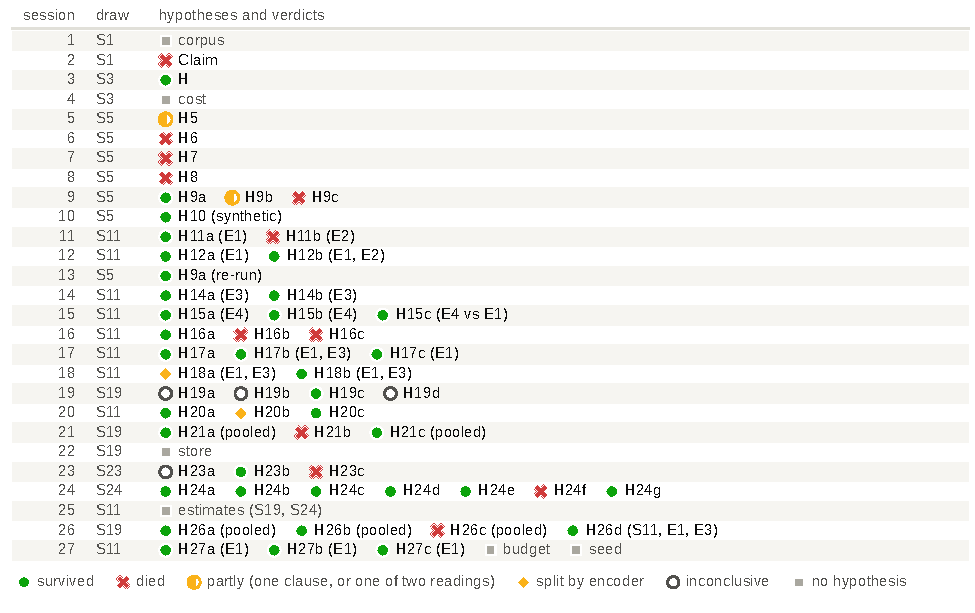
\includegraphics[width=\textwidth]{figures/fig_study.pdf}
\caption{The study as it ran. Each row is a session with the draw it scored: Zenodo records (S1 to S11), GitHub directories (S19, S24) or whole repository trees (S23). A marker gives the verdict of one pre-registered hypothesis, stated with its criterion in the appendix. On S11 a label names the encoders a hypothesis was read under, or none when it was read under all four. On the GitHub draws and the trees every hypothesis was read under E1, and H21a and H21c take the pooled reading of both GitHub draws, as the brief of session 24 fixed. Session 26 was registered after an earlier round of review, on draws already read. H26a to H26c pool the two GitHub draws, and H26d is on S11. Session 27 was registered after a later round of review. Its H27a to H27c are read on queries that a model wrote as a simulated searcher, and its budget and seed readings have no kill criterion. Squares mark the sessions, or the parts of a session, that tested no hypothesis.}
\label{fig:study}
\end{figure}

\section{Pooling loses the minority modality}
\label{sec:loss}

\paragraph{The exploratory finding.} The study began with a different claim, that pooling collapses a directory toward its text and loses image-heavy children. On S1 that claim died under its kill criterion, which needed the pooled centroid beaten on image queries in both image-heavy buckets. It was beaten in $[.5,.8)$ (\rep{c} minus \rep{a} $+0.054$) and not in $[.8,1]$ ($-0.001$ \ci{-0.020}{+0.016}). The same tables showed a different pattern. The pooled centroid lost 0.27 recall@5 on image queries in the most text-heavy directories and 0.27 on text-like queries in the most image-heavy ones, and almost nothing where the query's modality dominated its directory ($-0.001$ and $+0.021$). What the pooled vector loses is the \emph{minority} modality of each directory, whichever modality that is.

\paragraph{Pre-registered on fresh directories.} The pattern was then written down as a hypothesis with its cells and kill rule and tested on S3, 400 directories drawn after S1 was excluded. It survived, with \rep{c} minus \rep{a} at $+0.179$ \ci{+0.115}{+0.251} in P1 and $+0.200$ \ci{+0.135}{+0.270} in P2 ($+0.188$ and $+0.197$ when S3 is re-scored under the later .xls rule). The per-modality centroids \rep{b} gain the same ($+0.184$, $+0.195$). In the majority cells \rep{c}'s gain is $+0.045$ and $+0.008$. On the main set S5, where these cells were a reported secondary rather than a kill test, the loss is larger and the intervals are tight, at $+0.238$ \ci{+0.207}{+0.268} and $+0.233$ \ci{+0.207}{+0.262} over all 23,130 queries. On the confirmation set S11 under E1 it is $+0.253$ \ci{+0.214}{+0.294} and $+0.169$ \ci{+0.136}{+0.200}. The kill tests of the loss on S11 are the E2, E3 and E4 measurements, the second calibration seed below and the checks of Section~\ref{sec:validity}. Table~\ref{tab:loss} and Figure~\ref{fig:loss} collect the six measurements, and Table~\ref{tab:cells} gives the cells on S11.

\begin{figure}[t]
\centering
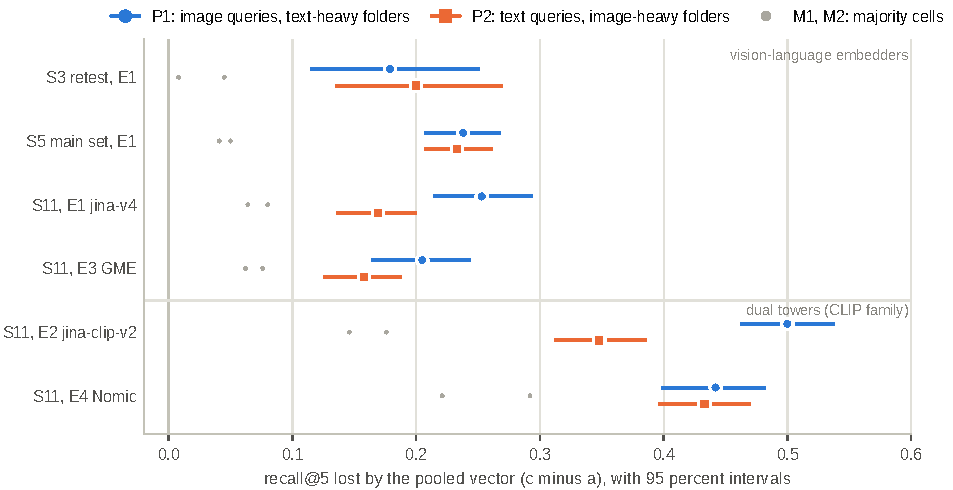
\includegraphics[width=\textwidth]{figures/fig_loss.pdf}
\caption{How much the pooled vector loses: recall@5 of \rep{c} minus \rep{a} with paired 95 percent intervals, for every measurement in Table~\ref{tab:loss}. Blue: image queries in text-heavy folders (P1). Orange: text queries in image-heavy folders (P2). Gray: the majority cells (M1, M2). The upper rows are vision-language embedders and the lower rows CLIP-family dual towers.}
\label{fig:loss}
\end{figure}

\begin{table}[t]
\centering\small
\caption{The minority-modality loss, recall@5 of \rep{c} minus \rep{a}, paired bootstrap over directories. P1: image queries in text-heavy directories; P2: text-like queries in image-heavy directories; M1 and M2: the majority cells. Kill-tested rows are marked. The S11 row under E1 was kill-tested under a second calibration seed ($+0.255$ and $+0.193$).}
\label{tab:loss}
\resizebox{\textwidth}{!}{%
\begin{tabular}{llrrrr}
\toprule
Set & Encoder & P1 & P2 & M1 & M2 \\
\midrule
S3 (kill-tested) & E1 & $+0.179$ \ci{+0.115}{+0.251} & $+0.200$ \ci{+0.135}{+0.270} & $+0.045$ & $+0.008$ \\
S5 (main, 2,808 dirs; reported) & E1 & $+0.238$ \ci{+0.207}{+0.268} & $+0.233$ \ci{+0.207}{+0.262} & $+0.041$ & $+0.050$ \\
S11 (reported; second seed kill-tested) & E1 & $+0.253$ \ci{+0.214}{+0.294} & $+0.169$ \ci{+0.136}{+0.200} & $+0.080$ & $+0.064$ \\
S11 (kill-tested) & E2 (jina-clip) & $+0.500$ \ci{+0.462}{+0.538} & $+0.348$ \ci{+0.312}{+0.386} & $+0.146$ & $+0.176$ \\
S11 (kill-tested) & E3 (GME) & $+0.205$ \ci{+0.164}{+0.244} & $+0.158$ \ci{+0.125}{+0.188} & $+0.076$ & $+0.062$ \\
S11 (kill-tested) & E4 (Nomic) & $+0.442$ \ci{+0.398}{+0.482} & $+0.433$ \ci{+0.396}{+0.470} & $+0.292$ & $+0.221$ \\
\bottomrule
\end{tabular}}
\end{table}

\begin{table}[t]
\centering\small
\caption{Recall@5 on the S11 evaluation split (17,140 queries over 2,035 directories, 2,597 ranked) by representation, encoder and cell; the cells hold 1,959 (P1), 2,146 (P2), 5,571 (M1) and 7,272 (M2) queries under every encoder. Vision-language embedders above, dual towers below. Vectors per directory in parentheses. \rep{a}: pooled; \rep{ac}: pooled, centered; \rep{bc2}: two labelled centered centroids; \rep{tb2c}: two blind centered clusters; \rep{c}: per-modality $k$-reps; \rep{cc}: the same, centered; \rep{d}: every file; \rep{dc}: every file, centered.}
\label{tab:cells}
\setlength{\tabcolsep}{4pt}
\begin{tabular}{lrrrrrrrrrr}
\toprule
& \multicolumn{5}{c}{E1 jina-embeddings-v4} & \multicolumn{5}{c}{E3 gme-Qwen2-VL-2B} \\
\cmidrule(lr){2-6}\cmidrule(lr){7-11}
 & all & P1 & P2 & M1 & M2 & all & P1 & P2 & M1 & M2 \\
\midrule
\rep{a} (1.00) & 0.692 & 0.421 & 0.370 & 0.730 & 0.830 & 0.716 & 0.536 & 0.386 & 0.761 & 0.827 \\
\rep{ac} (1.00) & 0.719 & 0.513 & 0.474 & 0.734 & 0.835 & 0.731 & 0.552 & 0.471 & 0.768 & 0.826 \\
\rep{bc2} (1.95) & 0.769 & 0.671 & 0.591 & 0.773 & 0.845 & 0.782 & 0.709 & 0.593 & 0.812 & 0.833 \\
\rep{tb2c} (2.00) & 0.781 & 0.638 & 0.575 & 0.805 & 0.862 & 0.788 & 0.682 & 0.565 & 0.831 & 0.849 \\
\rep{c} (5.20) & 0.796 & 0.674 & 0.539 & 0.810 & 0.894 & 0.811 & 0.741 & 0.544 & 0.837 & 0.889 \\
\rep{cc} (5.20) & 0.810 & 0.713 & 0.590 & 0.814 & 0.899 & 0.816 & 0.742 & 0.568 & 0.839 & 0.890 \\
\rep{d} (9.87) & 0.804 & 0.685 & 0.551 & 0.821 & 0.897 & 0.815 & 0.744 & 0.547 & 0.843 & 0.890 \\
\rep{dc} (9.87) & 0.818 & 0.714 & 0.597 & 0.828 & 0.905 & 0.820 & 0.745 & 0.569 & 0.847 & 0.894 \\
\midrule
 & \multicolumn{5}{c}{E2 jina-clip-v2} & \multicolumn{5}{c}{E4 Nomic Embed v1.5} \\
\cmidrule(lr){2-6}\cmidrule(lr){7-11}
 & all & P1 & P2 & M1 & M2 & all & P1 & P2 & M1 & M2 \\
\midrule
\rep{a} (1.00) & 0.457 & 0.055 & 0.035 & 0.640 & 0.551 & 0.397 & 0.006 & 0.005 & 0.397 & 0.621 \\
\rep{ac} (1.00) & 0.559 & 0.278 & 0.229 & 0.702 & 0.624 & 0.544 & 0.082 & 0.189 & 0.572 & 0.756 \\
\rep{bc2} (1.95) & 0.617 & 0.538 & 0.390 & 0.734 & 0.615 & 0.633 & 0.421 & 0.451 & 0.616 & 0.762 \\
\rep{tb2c} (2.00) & 0.634 & 0.450 & 0.331 & 0.778 & 0.664 & 0.640 & 0.331 & 0.398 & 0.657 & 0.788 \\
\rep{c} (5.20) & 0.683 & 0.555 & 0.383 & 0.786 & 0.727 & 0.693 & 0.448 & 0.438 & 0.689 & 0.842 \\
\rep{cc} (5.20) & 0.693 & 0.575 & 0.404 & 0.786 & 0.737 & 0.703 & 0.460 & 0.465 & 0.693 & 0.850 \\
\rep{d} (9.87) & 0.694 & 0.554 & 0.383 & 0.796 & 0.745 & 0.705 & 0.460 & 0.456 & 0.702 & 0.850 \\
\rep{dc} (9.87) & 0.706 & 0.570 & 0.401 & 0.798 & 0.761 & 0.715 & 0.470 & 0.466 & 0.715 & 0.858 \\
\bottomrule
\end{tabular}
\end{table}

\paragraph{Under CLIP-family dual towers the loss is larger.} Under E2 the pooled centroid finds the directory of a minority-modality query in the top five 5.5 percent (P1) and 3.5 percent (P2) of the time, against 55.5 and 38.3 percent for \rep{c}. That makes \rep{c} minus \rep{a} $+0.500$ \ci{+0.462}{+0.538} and $+0.348$ \ci{+0.312}{+0.386}. The majority cells lose too ($+0.146$, $+0.176$). Session 15 added E4, a second dual tower from another vendor, and tested the loss on S11 by the same rule (H15a). It survived, at $+0.442$ \ci{+0.398}{+0.482} in P1 and $+0.433$ \ci{+0.396}{+0.470} in P2. Under E4 the pooled centroid finds the directory of a minority-modality query in the top five 0.6 and 0.5 percent of the time, against 0.2 percent for a random ranking. Its majority cells lose $+0.292$ and $+0.221$. The session also pre-registered that on the same queries the loss under E4 exceeds the loss under E1 (H15c). The paired difference is $+0.189$ \ci{+0.145}{+0.231} in P1 and $+0.265$ \ci{+0.226}{+0.305} in P2, so H15c survived. Measured the same way, E2 loses more than E1 by $+0.247$ \ci{+0.208}{+0.286} and $+0.179$ \ci{+0.142}{+0.223}. Between the two towers the order depends on the cell. E4 loses less than E2 in P1 ($-0.058$ \ci{-0.088}{-0.025}) and more in P2 ($+0.086$ \ci{+0.067}{+0.105}). The two towers are also the weakest encoders of the four on these files, by the pilot check and by \rep{c} over all queries (0.683 under E2 and 0.693 under E4, against 0.796 under E1 and 0.811 under E3). In the minority cells \rep{c} reaches 0.555 and 0.383 under E2 and 0.448 and 0.438 under E4, against 0.674 and 0.539 under E1 and 0.741 and 0.544 under E3. Part of the larger loss is therefore the encoders, and not only their wider gap.

\paragraph{Under a second vision-language embedder the loss holds.} E1 and E2 come from one vendor. Session 14 added E3, from another, and tested the loss on S11 under the kill rule of session 3, fixed in the brief before any E3 number was computed (H14a). It survived, with \rep{c} minus \rep{a} at $+0.205$ \ci{+0.164}{+0.244} in P1 and $+0.158$ \ci{+0.125}{+0.188} in P2. The majority cells lose $+0.076$ and $+0.062$. E3 is the strongest of the four encoders on these files over all queries (\rep{c} 0.811 against 0.796 under E1, 0.693 under E4 and 0.683 under E2). Its pooled centroid still finds the directory of an image query in a text-heavy folder in the top five only 53.6 percent of the time, against 74.1 percent for \rep{c}. The brief expected a loss between E1's and E2's if E3's gap lay between theirs. The gap is about E1's instead (0.369 against 0.381; Section~\ref{sec:mechanism}), and so is the loss (0.253 and 0.169 under E1).

\paragraph{Robust to the calibration split.} The S11 numbers use one 20 percent calibration split (seed 20261102) for the group means and the cell membership. Session 12 repeated the evaluation under a second seed (20261103; 17,208 queries over 2,034 directories) with the pre-registered expectation that the verdicts do not move. They do not. Under E1 \rep{c} minus \rep{a} is $+0.255$ \ci{+0.215}{+0.292} in P1 and $+0.193$ \ci{+0.163}{+0.228} in P2, and under E2 it is $+0.513$ \ci{+0.473}{+0.548} and $+0.361$ \ci{+0.325}{+0.395}, against $+0.253$, $+0.169$, $+0.500$ and $+0.348$ under the first seed. Every cell of \rep{tb2c} minus \rep{c} under E1 moves by at most 0.003 ($-0.035$ \ci{-0.058}{-0.012} in P1, $-0.029$ \ci{-0.043}{-0.017} in M2), so the two-vector verdict stands as reported, by the rule and by little.

\paragraph{The flat walk is the reference, and \rep{c} is close to it.} Keeping every file vector (\rep{d}) is the natural reference for a representation built from the same vectors. It is not a strict ceiling. On the full S5 set \rep{c} is 0.008 above it in M1 (interval \ci{0.001}{0.015}). On S11 \rep{cc} and \rep{dc} are above it in the minority cells under E1 and E2, and in P2 under E3 and E4. In P1 under E3 and E4, \rep{cc} is level with it. Over the five cells (all queries, P1, P2, M1, M2), \rep{c} is within 0.013 of \rep{d} on S3 and S5 and within 0.018 on S11 under all four encoders (Table~\ref{tab:cells}). This was pre-registered under E3 and E4 (H14b, H15b), where the largest gaps are 0.006 and 0.018. Under E4 \rep{c} is below \rep{d} in all five cells, with every interval below zero. In single-bucket cells the gap reaches 0.030. The useful question is therefore how much of file-level search a folder representation keeps.

\paragraph{The number of candidates.} The loss depends on how many folders compete. With the own folder and $n - 1$ others drawn at random as the candidates, the expected recall@5 follows from the ranks (session 25, post hoc). Under E1 on S11 the loss in P1 and P2 is $+0.014$ and $+0.032$ among 10 candidates, $+0.114$ \ci{+0.090}{+0.141} and $+0.140$ \ci{+0.119}{+0.164} among 100, and $+0.232$ and $+0.152$ among 1,000, against $+0.253$ and $+0.169$ among all 2,597. The GitHub draws are read the same way in Section~\ref{sec:github}.

\section{Searcher queries}
\label{sec:searcher}

Every query so far is a file of a folder or, in Section~\ref{sec:nlq}, the depositor's own words about a record. Session 27 asked whether the loss reaches the words someone would type to find one file again. Its brief drew the folders and the target files and built a tool for writing queries, and the author was to write them. The tool showed each folder's pictures as thumbnails and the first 300 characters of its documents, with file names, the record's title and description and every digit hidden. The author found the documents of the first folder, raw numeric data files, unreadable with their digits hidden, and no person wrote queries. An amendment, committed before any query was embedded or scored, made a language model the writer. The Bitcoin block that anchors its timestamp was mined a few minutes after the scoring run ended, so that order rests on the repository's history. The hypotheses and the scoring stayed as the brief fixed them, and the brief's block precedes every number of the session. Language models have written queries for retrieval before, as training data \citep{bonifacio2022inpars} and as query variants for test collections \citep{alaofi2023variants}. We report these as queries that a model wrote as a simulated searcher.

\paragraph{Folders and targets.} The folders are evaluation-split folders of the confirmation set outside the four digitization series of Section~\ref{sec:validity}. Each holds at least two images and two text-like files that are evaluation queries under E1 and have a vector under all four encoders. A fixed seed drew 30 folders per image-fraction bucket, at most one per creator family, 120 in all. In each folder one image and one text-like file were drawn as targets, with further files in a drawn order in case the writer could not describe a target. The writer therefore could not pick the files a pooled vector misses. The sample was committed before any query was written.

\paragraph{The writer.} Claude Opus 5.5 (Anthropic) wrote the queries, as six subagents of the assistant that ran the session, each given twenty folders. Each subagent saw a prompt that says nothing about the study, its representations, its hypotheses or any result, and the material the tool shows for its folders. That material is a sheet of every picture in the folder with the target framed, the target pictures at the tool's size, and the folder's documents as the tool shows them, digits hidden. For each folder a subagent wrote one query to find the target picture (QI) and one to find the target document (QT), as the words someone would type into a search box. A script checked the tool's rules on every query, no digit and no run of five words copied from the folder's text, and all 200 queries pass both. Their median length is eight words. One picture target and one document target were skipped as impossible to describe. The subagent given 20 of the folders was refused by an automated permission check before it ran and was not retried. That leaves 100 folders, 25 per bucket, and 50 queries in each of four cells. The writer belongs to none of the encoders' model families.

\paragraph{Scoring.} Each query is embedded on its encoder's query text path, as the titles of Section~\ref{sec:nlq} are. Every one of the 2,597 confirmation folders is a candidate, represented by all of its files with a vector, since the query is not a file. The minority cells are QI-T, picture queries for folders with image fraction below 0.5, and QT-I, document queries for folders at 0.5 or more. Their majority counterparts are QI-I and QT-T. Intervals are 95 percent from 1,000 resamples of creator families, and with one folder per family a cell holds 50 families. Before any query was scored, the scorer reproduced the ranks of \rep{a}, \rep{c} and \rep{d} on all 2,597 titles of Section~\ref{sec:nlq} under each encoder. On the queries, the flat walk \rep{d} reaches recall@5 0.720 in QI-T and 0.940 in QT-I under E1, above the 0.25 below which the brief would have read a cell's queries as too vague.

\paragraph{The loss.} Three hypotheses were registered under E1 (Figure~\ref{fig:searcher}). H27a required \rep{c} minus \rep{a} of at least $+0.05$ in QI-T with its interval above zero, and it survived at $+0.140$ \ci{+0.020}{+0.280}. H27b, the same in QT-I, survived at $+0.420$ \ci{+0.280}{+0.560}. H27c read \rep{c} minus \rep{d} over all 200 queries as non-inferiority at the margin of 0.02, and at $+0.000$ \ci{-0.020}{+0.020} it is not inferior. Over all queries the pooled vector reaches recall@5 0.675, and \rep{c} and \rep{d} reach 0.870. In QT-I the pooled vector reaches 0.500 against 0.920 for \rep{c}, and in QI-T 0.600 against 0.740. The brief reads H27a and H27b together as an intersection-union test \citep{berger1982iut}, each on its 95 percent interval. Counted instead as one family of three primary tests, H27a's 98.33 percent interval runs from $-0.020$ to $+0.314$ and reaches below zero, so that reading would call it dead. H27b's runs from $+0.260$ to $+0.594$, and H27c's from $-0.025$ to $+0.020$, which that reading would call inconclusive.

\begin{figure}[t]
\centering
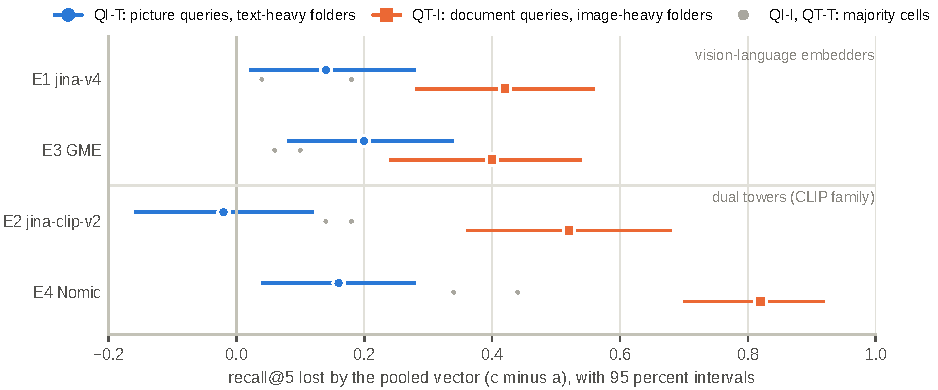
\includegraphics[width=\textwidth]{figures/fig_searcher.pdf}
\caption{The loss on queries that a model wrote as a simulated searcher (session 27): recall@5 of \rep{c} minus \rep{a} with creator-clustered 95 percent intervals, 50 queries per cell from 100 folders of the confirmation set, all 2,597 folders ranked. Blue: picture queries in text-heavy folders (QI-T). Orange: document queries in image-heavy folders (QT-I). Gray: the majority cells (QI-I, QT-T). The registered tests are the E1 rows.}
\label{fig:searcher}
\end{figure}

\paragraph{Other encoders and cells.} Under the other three encoders the document cell loses as well, by $+0.520$ under E2, $+0.400$ under E3 and $+0.820$ under E4, with every interval above zero. The picture cell loses under E3 and E4, by $+0.200$ \ci{+0.080}{+0.340} and $+0.160$ \ci{+0.040}{+0.280}, and shows no loss under E2 ($-0.020$ \ci{-0.160}{+0.120}). Under E1 a document query also loses in text-heavy folders, $+0.180$ \ci{+0.080}{+0.300} in QT-T, as titles do (Section~\ref{sec:nlq}), and a picture query in an image-heavy folder loses little ($+0.040$ \ci{-0.060}{+0.140}). Centering does not help the pooled vector under E1 ($-0.010$ \ci{-0.040}{+0.020} over all queries). Two blind clusters lose against \rep{c}, by $0.110$ \ci{0.060}{0.165} centered and $0.090$ \ci{0.045}{0.140} uncentered.

\paragraph{File names.} The writer saw no file name. A router that scores a folder by the best character $n$-gram cosine between the query and its files' names, built as in Section~\ref{sec:validity}, puts the target's folder in the top five for 0.240 of the queries. Fused with the E1 vector rankings by reciprocal rank fusion ($k = 60$), \rep{c} minus \rep{a} is $+0.090$ \ci{+0.045}{+0.135} over all queries and $+0.220$ \ci{+0.100}{+0.340} in QT-I.

\paragraph{What these queries can show.} A model wrote them, from what a person would see of a folder, and a model's queries may be more specific than a person's. In a study of test-collection queries, variants written by a language model found similar sets of relevant documents to people's variants without capturing their full variety \citep{alaofi2023variants}. Fifty queries per cell is a small sample, and the interval of the picture cell reaches down to 0.02. The result shows the loss on queries written to find one file from what is visible of its folder, in both cells under E1, E3 and E4 and in the document cell under E2. Whether it appears on the queries of people searching their own folders was not measured.

\section{The mechanism: a folder is two clusters}
\label{sec:mechanism}

The obvious explanation is the modality gap \citep{liang2022mindgap}. If a folder's images and texts sit in different regions, their mean sits in neither, and a query of the smaller group is far from it. We tested the published remedy, per-modality mean-centering before pooling \citep{li2025grclip}, as a pre-registered hypothesis on S5. It said that the centered pooled centroid \rep{ac}, still one vector per folder, recovers more than half of what \rep{c} recovers. From here on, S5 numbers are on its evaluation split (18,742 queries; the calibration split supplies the group means), where \rep{c} minus \rep{a} is $+0.236$ and $+0.241$.

\paragraph{Centering closes most of the global gap and leaves each folder split.} The distance between the mean image-input vector and the mean text-input vector over the evaluation split falls from 0.361 to 0.072 after centering. The folders do not follow. Table~\ref{tab:gap} and Figure~\ref{fig:cosines} give the mean cosine of same-folder file pairs. Before centering, a cross-modality pair in the same folder has cosine 0.524, against 0.770 and 0.722 within a modality. After centering all three fall, the cross pairs most, to 0.205 against 0.568 and 0.462. Centering removes the shared offset between the two groups and leaves the within-folder separation, so the pooled vector still sits between two clusters. Under E2 the gap is wider, 0.787 before centering, and the same-folder cross cosine starts lower, at 0.196 against 0.751 and 0.701 within a modality (0.096 against 0.561 and 0.410 after centering). Under E3 the gap is 0.369, about E1's, and the folder is again two clusters, at 0.272 across against 0.611 and 0.569 within a modality (0.174 against 0.543 and 0.439 after centering). By these cosines E3 holds a folder's two groups further apart than E1 does, yet its loss is a little smaller. Under E4 the gap is the widest of the four, 1.095, and a folder's images and texts are close to orthogonal, at 0.066 across against 0.917 and 0.698 within a modality (0.034 against 0.555 and 0.406 after centering). Yet in P1 E4 loses less than E2 does (Section~\ref{sec:loss}). With four encoders we do not try to say what sets the size of the loss. Two published results on single items sit beside this. \citet{liu2026geometry} report that mean-centering takes the distance between the modality centroids from 0.686 to 0.020 and leaves what they call the distribution gap unchanged at 0.685. The folder-level cosines above show the same pattern inside folders, where the offset goes and the separation stays. \citet{li2025grclip} report that after centering, an interpolation of the image and the text embedding of one document beats either alone. A folder's files are not two views of one document. For them centering recovers part of the loss, about half on the main set, and no interpolation weight there recovers the rest (Section~\ref{sec:remedy}). The alignment score of 0.71 that \citet{gunther2025jinav4} report for E1 is the average cosine of matched image-text pairs, a different quantity from the distance between the modality means measured here.

\begin{figure}[t]
\centering
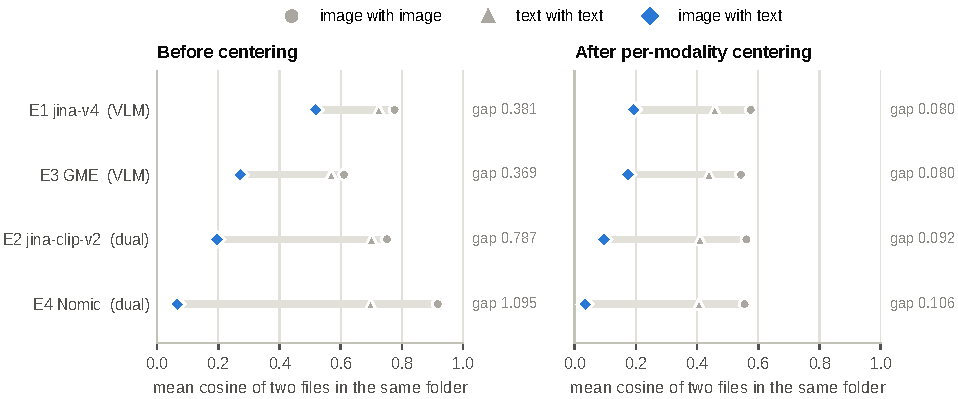
\includegraphics[width=\textwidth]{figures/fig_cosines.pdf}
\caption{A folder is two clusters under every encoder. Each row gives the mean cosine between two files of the same S11 folder: two images (circle), two texts (triangle), or an image and a text (blue diamond), before and after per-modality centering (Table~\ref{tab:gap}). The image-text pair sits well below both within-modality pairs, also after centering has closed most of the global gap (right-hand labels). In the row labels, VLM marks the vision-language embedders and dual the dual towers.}
\label{fig:cosines}
\end{figure}

\begin{table}[t]
\centering\small
\caption{The modality gap at folder level. Gap: norm of the mean image-input vector minus the mean text-input vector over the evaluation split. Cosines: mean over same-folder file pairs.}
\label{tab:gap}
\begin{tabular}{llrrrr}
\toprule
Set, encoder & Vectors & Gap & img-img & txt-txt & img-txt \\
\midrule
S5, E1 & uncentered & 0.361 & 0.770 & 0.722 & 0.524 \\
S5, E1 & centered & 0.072 & 0.568 & 0.462 & 0.205 \\
S11, E1 & uncentered & 0.381 & 0.776 & 0.725 & 0.518 \\
S11, E1 & centered & 0.080 & 0.575 & 0.458 & 0.193 \\
S11, E2 & uncentered & 0.787 & 0.751 & 0.701 & 0.196 \\
S11, E2 & centered & 0.092 & 0.561 & 0.410 & 0.096 \\
S11, E3 & uncentered & 0.369 & 0.611 & 0.569 & 0.272 \\
S11, E3 & centered & 0.080 & 0.543 & 0.439 & 0.174 \\
S11, E4 & uncentered & 1.095 & 0.917 & 0.698 & 0.066 \\
S11, E4 & centered & 0.106 & 0.555 & 0.406 & 0.034 \\
\bottomrule
\end{tabular}
\end{table}

\paragraph{Centering recovers part of the loss, and balancing trades the majority for the minority.} The hypothesis died. On S5, \rep{ac} recovers 49 percent of \rep{c}'s gain over \rep{a} in both minority cells ($(\rep{ac} - \rep{a}) - 0.5(\rep{c} - \rep{a}) = -0.002$ \ci{-0.023}{+0.018} in P1 and $-0.001$ \ci{-0.020}{+0.019} in P2). On S11 centering recovers 36 and 62 percent under E1, 45 and 56 percent under E2, 8 and 54 percent under E3 and 17 and 42 percent under E4. Under E3 it does almost nothing for image queries in text-heavy folders (\rep{ac} minus \rep{a} is 0.016 of the 0.205 in P1). On S5 a balanced one-vector folder (\rep{ab}, the mean of the two group means) recovers 92 to 93 percent of the minority loss, and a centered balanced vector (\rep{acb}) 107 to 110 percent. Both pay in the majority cells, where \rep{ab} changes recall@5 by $-0.030$ and $-0.069$ against the pooled centroid and \rep{acb} by $-0.025$ and $-0.048$ (against \rep{c}, $-0.071$ and $-0.113$, $-0.065$ and $-0.092$). In the single-modality-heavy buckets the cost reaches $-0.149$. No single vector we tried held both the minority and the majority. Centering also helps the multi-vector representation and the flat walk itself, so its benefit is not specific to folder vectors. On the S5 evaluation queries \rep{cc} minus \rep{c} is $+0.017$ and \rep{dc} minus \rep{d} $+0.018$, with $+0.037$ to $+0.047$ in the minority cells. Under E3 on S11 the gains are $+0.004$ and $+0.006$ over all queries, $+0.022$ to $+0.025$ in P2 and nothing in P1. Under E4 both are $+0.010$ over all queries and $+0.010$ to $+0.027$ in the minority cells.

\section{Modality, or any minority?}
\label{sec:dilution}

A sharper objection is that nothing above is about modality. A pooled mean dilutes any minority, and a folder's minority modality is simply a minority. On natural folders the two cannot be separated, because label-blind clustering of a folder's files recovers the modality partition. On S5 the blind clusters are 0.88 to 0.99 pure by input group. A pre-registered hypothesis, H9c, was that \rep{c} beats blind $k$-means at its own budget in both minority cells. It died, at $+0.000$ \ci{-0.005}{+0.006} and $+0.001$ \ci{-0.005}{+0.006}, and the test could not tell modality from dilution. We therefore built the control directly. Hosts are evaluation-split directories of S5 with at least six files, all of one input group. Into each host we planted a guest set of files from one other single-group record, at a fraction drawn uniformly from $[0.2, 0.5)$. We did this once with a record of the same input group (set SAME) and once with a record of the other group (set CROSS), at the same fraction for a host in both sets. Nothing is fitted on the synthetic folders. The pre-registered hypothesis is that the pooled centroid loses more on guest queries in CROSS than in SAME.

The corpus was selected for mixed folders, so the control is small. The evaluation split has 31 single-group directories of host size, donors come from the same pool, and 20 hosts received a guest in SAME, 16 of them also in CROSS. On the 10 hosts with guest queries in both sets, the loss of \rep{a} against \rep{d} on guest queries is 0.763 in CROSS and 0.583 in SAME. The difference is $+0.180$ \ci{+0.021}{+0.345}, so the hypothesis survives, by little. The guest also costs the host, with $+0.118$ \ci{+0.026}{+0.238} more loss on the host's own queries when the guest is of the other modality (16 hosts). Two things in the control matter more than the verdict. First, most of the control's loss is there with no modality difference at all. On those ten hosts a same-modality minority from another record costs the pooled centroid 0.58 recall@5 on its queries, three quarters of the cross-modality 0.76 (over each set's own hosts, 0.50 on 19 against 0.71 on 11). A pooled vector loses any foreign minority of a fifth to a half of the folder, and the modality adds 0.18 on top. Second, the labelled two-centroid representation cannot see a same-modality minority. Its SAME loss, 0.52, is no better than the pooled centroid's 0.50. Two label-blind clusters recover most of it in both sets (losses of 0.11 in SAME and 0.02 in CROSS, and 0.16 and 0.10 when centered). The guests here are topically foreign in a way a natural minority modality is not. Both synthetic losses are therefore two to three times the natural 0.24 to 0.25 (\rep{d} minus \rep{a} in P1 and P2 on the S5 evaluation split), and their ratio does not decompose the natural loss. Ten hosts is a small sample, and the interval's lower end is 0.021. A larger version of this control needs a corpus with single-modality folders of its own.

\section{The loss reaches natural-language queries}
\label{sec:nlq}

The file queries of Sections~\ref{sec:loss}, \ref{sec:mechanism} and~\ref{sec:dilution} measure whether a folder vector represents its own files. Session 12 asked, pre-registered, whether the same vectors answer a text query that is not a file. One query is the Zenodo record's title (Q\textsubscript{title}, 2,597 queries, one per S11 directory). The other is the title followed by the record's description from the Zenodo metadata (Q\textsubscript{desc}, the 2,399 records with a non-empty description, median 842 characters, cut by the study's 2,000-token input rule like every text input). The relevant folder is the record's own directory. Every directory is a candidate, and the representations are built from all of a directory's embedded files, since the query is not one of them. The centered rows subtract the calibration split's text-input mean from the query, and nothing is fitted on the queries. The hypothesis H12a was that the pooled centroid loses to \rep{c} on image-heavy directories (image fraction at least 0.5) on Q\textsubscript{title} under E1. It survived, at $+0.182$ \ci{+0.158}{+0.206} recall@5, with $+0.263$ \ci{+0.236}{+0.290} under E2 and $+0.231$ \ci{+0.204}{+0.256} and $+0.359$ \ci{+0.333}{+0.389} on Q\textsubscript{desc}. Session 14 ran the same queries under E3, with no instruction on the query as on the files, and found $+0.218$ \ci{+0.190}{+0.244} on Q\textsubscript{title} and $+0.189$ \ci{+0.163}{+0.216} on Q\textsubscript{desc}. Session 15 ran them under E4, with the query prefix used on the files, and found $+0.548$ \ci{+0.522}{+0.577} on titles and $+0.555$ \ci{+0.526}{+0.584} on descriptions. Under E4 the pooled centroid finds an image-heavy folder from its title in the top five 0.7 percent of the time. Table~\ref{tab:nlq} gives the levels.

\begin{table}[t]
\centering\small
\caption{Recall@5 with the record's title (Q\textsubscript{title}, 2,597 queries) or title and description (Q\textsubscript{desc}, 2,399 queries, the records with a non-empty description) as the query, at most one query per S11 record, all 2,597 directories ranked. T: text-heavy directories (image fraction below 0.5; 1,215 and 1,156 queries); I: image-heavy (1,382 and 1,243). Random recall@5 is 0.002. Vision-language embedders above, dual towers below; vectors per directory in parentheses. \rep{a}: pooled; \rep{ac}: pooled, centered (files and query); \rep{tb2}: two blind clusters; \rep{tb2c}: the same, centered; \rep{c}: per-modality $k$-reps; \rep{cc}: the same, centered; \rep{d}: every file.}
\label{tab:nlq}
\setlength{\tabcolsep}{4pt}
\begin{tabular}{lrrrrrrrrrrrr}
\toprule
& \multicolumn{6}{c}{E1 jina-embeddings-v4} & \multicolumn{6}{c}{E3 gme-Qwen2-VL-2B} \\
\cmidrule(lr){2-7}\cmidrule(lr){8-13}
 & \multicolumn{3}{c}{Q\textsubscript{title}} & \multicolumn{3}{c}{Q\textsubscript{desc}} & \multicolumn{3}{c}{Q\textsubscript{title}} & \multicolumn{3}{c}{Q\textsubscript{desc}} \\
\cmidrule(lr){2-4}\cmidrule(lr){5-7}\cmidrule(lr){8-10}\cmidrule(lr){11-13}
 & all & T & I & all & T & I & all & T & I & all & T & I \\
\midrule
\rep{a} (1.00) & 0.658 & 0.718 & 0.606 & 0.708 & 0.797 & 0.626 & 0.582 & 0.662 & 0.512 & 0.662 & 0.723 & 0.606 \\
\rep{ac} (1.00) & 0.656 & 0.682 & 0.633 & 0.743 & 0.781 & 0.708 & 0.630 & 0.648 & 0.615 & 0.701 & 0.698 & 0.704 \\
\rep{tb2} (2.00) & 0.742 & 0.729 & 0.753 & 0.813 & 0.798 & 0.826 & 0.674 & 0.656 & 0.690 & 0.741 & 0.719 & 0.762 \\
\rep{tb2c} (2.00) & 0.727 & 0.714 & 0.737 & 0.824 & 0.804 & 0.843 & 0.693 & 0.659 & 0.722 & 0.754 & 0.718 & 0.788 \\
\rep{c} (5.20) & 0.792 & 0.796 & 0.788 & 0.850 & 0.843 & 0.857 & 0.718 & 0.705 & 0.729 & 0.776 & 0.755 & 0.795 \\
\rep{cc} (5.20) & 0.777 & 0.777 & 0.776 & 0.860 & 0.845 & 0.874 & 0.733 & 0.708 & 0.755 & 0.788 & 0.762 & 0.813 \\
\rep{d} (9.87) & 0.794 & 0.796 & 0.792 & 0.854 & 0.845 & 0.862 & 0.722 & 0.710 & 0.733 & 0.780 & 0.762 & 0.797 \\
\midrule
 & \multicolumn{6}{c}{E2 jina-clip-v2} & \multicolumn{6}{c}{E4 Nomic Embed v1.5} \\
\cmidrule(lr){2-7}\cmidrule(lr){8-13}
 & \multicolumn{3}{c}{Q\textsubscript{title}} & \multicolumn{3}{c}{Q\textsubscript{desc}} & \multicolumn{3}{c}{Q\textsubscript{title}} & \multicolumn{3}{c}{Q\textsubscript{desc}} \\
\cmidrule(lr){2-4}\cmidrule(lr){5-7}\cmidrule(lr){8-10}\cmidrule(lr){11-13}
 & all & T & I & all & T & I & all & T & I & all & T & I \\
\midrule
\rep{a} (1.00) & 0.429 & 0.549 & 0.324 & 0.413 & 0.600 & 0.238 & 0.205 & 0.431 & 0.007 & 0.240 & 0.492 & 0.005 \\
\rep{ac} (1.00) & 0.378 & 0.430 & 0.331 & 0.496 & 0.533 & 0.463 & 0.399 & 0.562 & 0.255 & 0.476 & 0.631 & 0.331 \\
\rep{tb2} (2.00) & 0.565 & 0.523 & 0.603 & 0.602 & 0.574 & 0.627 & 0.563 & 0.554 & 0.572 & 0.621 & 0.623 & 0.619 \\
\rep{tb2c} (2.00) & 0.455 & 0.472 & 0.439 & 0.586 & 0.567 & 0.605 & 0.566 & 0.577 & 0.556 & 0.627 & 0.641 & 0.613 \\
\rep{c} (5.20) & 0.619 & 0.655 & 0.588 & 0.642 & 0.691 & 0.597 & 0.608 & 0.668 & 0.555 & 0.635 & 0.715 & 0.560 \\
\rep{cc} (5.20) & 0.527 & 0.587 & 0.474 & 0.634 & 0.659 & 0.611 & 0.631 & 0.675 & 0.593 & 0.683 & 0.734 & 0.636 \\
\rep{d} (9.87) & 0.629 & 0.675 & 0.588 & 0.653 & 0.714 & 0.597 & 0.628 & 0.686 & 0.577 & 0.660 & 0.739 & 0.587 \\
\bottomrule
\end{tabular}
\end{table}

\begin{figure}[t]
\centering
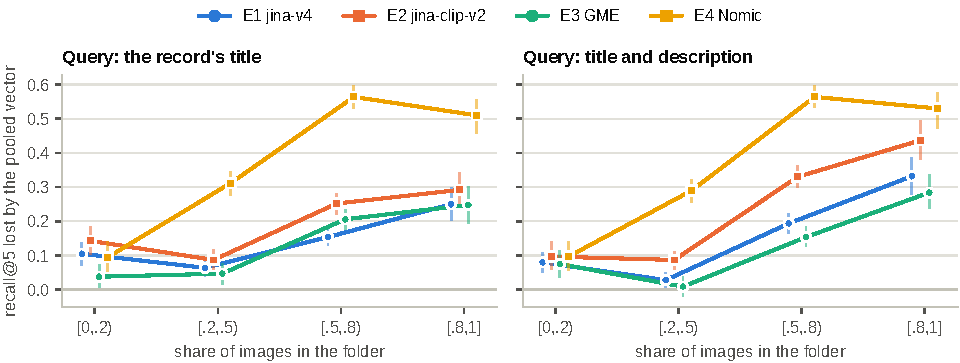
\includegraphics[width=\textwidth]{figures/fig_textq.pdf}
\caption{The loss with a text query that is not a file: recall@5 of \rep{c} minus \rep{a}, with 95 percent intervals, when the record's title (left) or its title and description (right) is the query, by the share of images in the folder. The loss is largest in image-heavy folders, since a text query reaches a folder through its text files.}
\label{fig:textq}
\end{figure}

Three things differ from the file-query picture (Figure~\ref{fig:textq}). First, the loss is on both sides of a text query. With a file as the query, the pooled centroid lost mostly where the query's modality was the directory's minority. With a text query it loses on text-heavy directories too, by less. Under E1 on Q\textsubscript{title}, \rep{c} minus \rep{a} is $+0.078$ \ci{+0.059}{+0.099} on text-heavy and $+0.182$ on image-heavy directories, and $+0.046$ and $+0.231$ on Q\textsubscript{desc}. Under E2 the pairs are $+0.106$ and $+0.263$, $+0.091$ and $+0.359$, under E3 $+0.044$ and $+0.218$, $+0.032$ and $+0.189$, and under E4 $+0.237$ and $+0.548$, $+0.223$ and $+0.555$. In six of the eight runs the loss is largest in the $[.8,1]$ bucket ($+0.248$ to $+0.437$). Under E4 it is largest in $[.5,.8)$, at $+0.564$ on both query sets, with $+0.510$ and $+0.530$ in $[.8,1]$. A text query reaches a directory through its text files, and the pooled vector of an image-heavy directory has few of them left. In five of the eight runs the loss is smallest in $[.2,.5)$. In $[0,.2)$, where fewer than one file in five is an image, it is still $+0.04$ to $+0.14$ (the smallest, under E3 on titles, with an interval reaching zero). That is the dilution of Section~\ref{sec:dilution}, among the directory's own texts.

Second, centering the query with the file-side text mean is not a dependable fix, and its effect depends on the encoder. On titles it does nothing under E1 (\rep{ac} minus \rep{a} $-0.002$ \ci{-0.012}{+0.008}), hurts under E2 ($-0.052$, and $-0.119$ on text-heavy directories) and helps under E3 and E4 ($+0.049$ \ci{+0.038}{+0.060} and $+0.193$ \ci{+0.177}{+0.209}). Where the query must cross the gap, on image-heavy directories, it helps on Q\textsubscript{desc} under all four encoders ($+0.082$, $+0.224$, $+0.098$ and $+0.327$) and on titles under E1, E3 and E4 ($+0.027$, $+0.103$ and $+0.248$). On text-heavy directories it does nothing or hurts in the six runs under E1 to E3 ($-0.014$ to $-0.119$). Under E4 it helps there too ($+0.131$ and $+0.138$), except in the most text-heavy bucket, where it does nothing. In no cell of Table~\ref{tab:nlq} does it reach \rep{c}. On image-heavy title queries \rep{ac} reaches 0.615 against 0.729 for \rep{c} under E3 and 0.255 against 0.555 under E4. The constant was fitted on file-side text inputs, whose mean is not the mean of a short title. A query-side constant would have to be fitted on held-out queries, which this study did not do by design.

Third, over all queries two vectors lose more against a text query than against a file under E1 and E2, about as much under E3 and less under E4. \rep{tb2c} is $0.065$ \ci{0.053}{0.078} below \rep{c} on Q\textsubscript{title} under E1 and $0.164$ under E2 ($0.026$ and $0.056$ on Q\textsubscript{desc}), against $0.015$ and $0.049$ with file queries. Under E3 it is $0.025$ \ci{0.012}{0.040} below on titles and $0.022$ on descriptions, against $0.023$ with files. Under E4 it is $0.042$ \ci{0.027}{0.057} below on titles and $0.008$ \ci{-0.009}{0.025} on descriptions, against $0.054$ with files. The uncentered pair \rep{tb2} is the better of the two on titles under E1 and E2 and on descriptions under E2. Under E3 and E4 the centered pair is ahead on both text query sets. With file queries it is ahead over all queries under E1 to E3 and level under E4 (0.640 each). Per-modality representatives stay close to the flat walk, less so under E4. Over all queries \rep{c} is within $0.011$ of \rep{d} in the six runs under E1 to E3 (\rep{d} minus \rep{c} $+0.002$ \ci{-0.002}{+0.007} under E1 and $+0.004$ \ci{-0.001}{+0.010} under E3 on Q\textsubscript{title}), at half the vectors. Under E4 it is $0.020$ \ci{0.013}{0.026} behind on titles and $0.025$ \ci{0.018}{0.033} on descriptions.

\section{Validity checks}
\label{sec:validity}

Two features of the corpus could inflate the loss. Files of one record often share a naming pattern or come in pairs, such as a figure and its PDF, and such siblings can make a folder easy to find from any one of its files. Some creators also deposited many records, so the directory bootstrap, which treats folders as independent, may give intervals that are too narrow. Session 17 tested both on S11 under all four encoders (Table~\ref{tab:validity}), with the hypotheses fixed before any loss on the new subsets was computed, and checked the evaluation code with a second implementation under E1.

\begin{table}[t]
\centering\small
\caption{The loss under creator clustering and on the clean subset (session 17, S11): recall@5 of \rep{c} minus \rep{a} in the minority cells, with 95 percent intervals from the directory bootstrap and from resampling creator families. The clean subset (750 P1 and 877 P2 queries) holds the queries whose folder a filename router misses, without a same-stem sibling and outside four digitization series. Its intervals are creator-clustered.}
\label{tab:validity}
\begin{tabular}{llrllrl}
\toprule
& & \multicolumn{3}{c}{All queries} & \multicolumn{2}{c}{Clean subset} \\
\cmidrule(lr){3-5}\cmidrule(lr){6-7}
Encoder & Cell & \rep{c} $-$ \rep{a} & Directories & Creators & \rep{c} $-$ \rep{a} & Creators \\
\midrule
E1 & P1 & $+0.253$ & \ci{+0.214}{+0.294} & \ci{+0.202}{+0.303} & $+0.128$ & \ci{+0.074}{+0.180} \\
 & P2 & $+0.169$ & \ci{+0.136}{+0.200} & \ci{+0.119}{+0.225} & $+0.172$ & \ci{+0.126}{+0.222} \\
E2 & P1 & $+0.500$ & \ci{+0.462}{+0.538} & \ci{+0.456}{+0.544} & $+0.323$ & \ci{+0.264}{+0.383} \\
 & P2 & $+0.348$ & \ci{+0.312}{+0.386} & \ci{+0.255}{+0.446} & $+0.298$ & \ci{+0.247}{+0.343} \\
E3 & P1 & $+0.205$ & \ci{+0.164}{+0.244} & \ci{+0.152}{+0.260} & $+0.095$ & \ci{+0.038}{+0.150} \\
 & P2 & $+0.158$ & \ci{+0.125}{+0.188} & \ci{+0.111}{+0.209} & $+0.163$ & \ci{+0.115}{+0.218} \\
E4 & P1 & $+0.442$ & \ci{+0.398}{+0.482} & \ci{+0.396}{+0.482} & $+0.248$ & \ci{+0.187}{+0.304} \\
 & P2 & $+0.433$ & \ci{+0.396}{+0.470} & \ci{+0.317}{+0.549} & $+0.391$ & \ci{+0.331}{+0.444} \\
\bottomrule
\end{tabular}
\end{table}

\paragraph{File names alone.} A router that sees only file names scores each folder by the best cosine between the name of the query file and the names of the folder's files, and ranks folders as the encoders do. It compares names by TF-IDF over character 3- and 4-grams of the lowercased base name, with the query file left out of its own folder. It puts the query's own folder in the top five for 0.700 of the evaluation queries, 0.617 in P1 and 0.587 in P2. The pooled E1 vector reaches 0.692. No encoder here reads a file name, but files whose names give their folder away may resemble their siblings in content as well. Session 26 fused the name ranking with the vector ranking by reciprocal rank fusion ($k = 60$, post hoc, registered before it ran). Under the two vision-language embedders the loss keeps about two fifths of its size, and under the dual towers most of it remains. Under E1 \rep{c} minus \rep{a} is then $+0.104$ \ci{+0.067}{+0.144} in P1 and $+0.067$ \ci{+0.041}{+0.097} in P2 (creator-clustered). Under E3 it is $+0.075$ \ci{+0.044}{+0.109} and $+0.057$ \ci{+0.035}{+0.086}, so H26d survived. Equal-weight fusion lifts the pooled vector (0.735 against 0.692 over all queries under E1) and the two dual towers. It lowers the representatives of the two vision-language embedders (0.780 against 0.796 under E1, 0.790 against 0.811 under E3). On GitHub, where the names alone reach 0.271 and 0.265, fusion nearly halves recall (0.706 to 0.387 for \rep{c} on the first draw, 0.646 to 0.361 on the second). The fused loss there is $+0.083$ \ci{+0.051}{+0.116} and $+0.067$ \ci{+0.044}{+0.091} in P1s and P2s, owner-weighted.

\paragraph{The clean subset.} A query is clean on three conditions. The filename router misses its folder (rank above five). Its folder holds no other file with the same stem and a different extension. Its record lies outside four digitization series, the deposits of four creator families that a count of P2 queries singled out before any loss was computed on them. H17b, pre-registered, required \rep{c} minus \rep{a} of at least $+0.05$ on the clean subset, with a creator-clustered interval above zero, in P1 and in P2 under E1 and under E3. It survived, and the same conditions hold under E2 and E4. On clean queries the image-query loss is about half of the loss over all queries under E1, E3 and E4 ($+0.128$ against $+0.253$, $+0.095$ against $+0.205$ and $+0.248$ against $+0.442$) and about two thirds of it under E2 ($+0.323$ against $+0.500$). The text-query loss does not shrink under E1 and E3 ($+0.172$ against $+0.169$ and $+0.163$ against $+0.158$) and shrinks a little under E2 and E4 ($+0.298$ against $+0.348$ and $+0.391$ against $+0.433$). Removing the four series alone raises it under all four encoders (to $+0.212$ under E1). The image queries whose folder the file names give away are 1,209 of the 1,959 in P1, and they lose more per query than the clean ones, so most of what the pooled vector loses on image queries is lost on them. That fits a lost match between sibling images, such as images of one series that resemble each other more than anything else. The subsets differ in other ways too, so this reading does not decompose the loss. In the majority cells the loss on clean queries is smaller as well, and under E1 the image-side one is gone ($-0.002$ \ci{-0.029}{+0.029} in M1, against $+0.080$ over all queries).

\paragraph{Creator-clustered intervals.} On the Zenodo sets, outside this section and Sections~\ref{sec:searcher} and~\ref{sec:abstracts}, the intervals in this paper resample directories. Here a record's family is its first creator, lowercased. The 2,597 S11 records come from 1,814 families, and about 47 effective families, the inverse of the summed squares of the families' shares of the queries, stand behind the 2,146 P2 queries (204 behind P1). Session 17 resampled each cell's families instead, 1,000 times, recomputing the difference over all queries of the drawn families. H17a, pre-registered, required the clustered interval of \rep{c} minus \rep{a} to lie above zero in P1 and in P2 under each encoder. It survived under all four. Of the two minority cells P2 widens more, to \ci{+0.317}{+0.549} under E4. The other verdicts re-read with clustered intervals do not move. The H15c differences stay above zero, as does E2 minus E1 (E4 minus E1: \ci{+0.142}{+0.239} in P1 and \ci{+0.184}{+0.346} in P2). No interval of \rep{c} minus \rep{d} lies entirely below $-0.02$ under any encoder. The lowest bound is $-0.027$, under E4 in P2, with an upper bound of $-0.010$. Under E1 \rep{tb2c} still passes the H11a rule (P1 \ci{-0.063}{-0.014}, M2 \ci{-0.064}{-0.010}). On S5 under E1 the clustered intervals of \rep{c} minus \rep{a} in the minority cells are \ci{+0.198}{+0.282} and \ci{+0.196}{+0.274}. With the title as the query, \rep{c} minus \rep{a} on image-heavy folders is $+0.182$ \ci{+0.126}{+0.242} under E1, and $+0.134$ \ci{+0.101}{+0.175} on the 744 image-heavy title queries that a filename router misses ($+0.239$, $+0.148$ and $+0.493$ under E2, E3 and E4). Weighting each family equally gives smaller estimates, with clustered intervals: under E1 $+0.133$ \ci{+0.103}{+0.163} in P1 and $+0.137$ \ci{+0.110}{+0.164} in P2, and on the clean subset $+0.059$ \ci{+0.025}{+0.094} and $+0.115$ \ci{+0.083}{+0.148}; under E3 $+0.105$ \ci{+0.079}{+0.135} and $+0.123$ \ci{+0.093}{+0.153}, and on the clean subset $+0.056$ \ci{+0.023}{+0.090} and $+0.096$ \ci{+0.060}{+0.132}. Creators with many queries contribute larger losses than the average creator. For image queries this is the most conservative reading the study offers, with creators counted once and the queries whose names give the folder away removed. Under it the image-query loss under the two vision-language embedders is about 0.06, with intervals that reach 0.02, below the smallest effect of interest of Section~\ref{sec:github}. Part of the drop under equal weighting comes from the lone files. With the query's folder holding a sibling of its input group (1,545 of the 1,959 P1 queries and 1,673 of the 2,146 P2 queries) the query-weighted loss under E1 is $+0.324$ and $+0.218$, and with families weighted equally $+0.266$ and $+0.239$ (Section~\ref{sec:github}).

\paragraph{A second implementation.} The earlier reproductions of the metric shared code with the evaluation script. For H17c an agent wrote a second implementation from a written specification, without reading the first one's code. On the E1 cache it gives the same rank as the evaluation script for every one of the 17,140 queries in rows \rep{a}, \rep{c} and \rep{d}.

\section{A second source: directories of GitHub repositories}
\label{sec:github}

Every folder above is a Zenodo record, from one search of one repository, selected for holding both an image type and a document type. Sessions 19 and 24 repeated the test on folders that people built for their own work, the directories of public GitHub repositories, on the conditions an earlier round of review of this study set for such a replication. Days from 2016 to 2025 were drawn at random, and for each day the pool holds the repositories created that day with at least five stars, as the GitHub search API returns them without a token \citep{github2026search}. A repository is usable if it is not a fork, is at most 200 MB and carries one of nine permissive licences (MIT, Apache-2.0, the two BSD licences, ISC, Unlicense, 0BSD, CC0-1.0 and CC-BY-4.0). A folder is a directory of the default branch at any depth with its direct children, read from the repository's tarball, outside hidden, vendored and dependency directories. Kept files follow the extension table and the 25 MB cap of the Zenodo sets. A directory with 3 to 100 kept files is eligible, and it is mixed if it keeps a file with an image extension and at least one other kept file. From each repository read, the scored set takes at most two mixed and two other eligible directories at random. Ground truth, input rules and representations are those of Section~\ref{sec:design}, with the same 20 percent calibration split by directory. The split's directories remain candidates and give no queries, so the evaluation queries below are fewer than the queries with a vector in Table~\ref{tab:corpora}.

The readings were tightened for this source. The minority cells keep only the queries whose folder still holds another file of the query's input group once the query is left out (P1s and P2s). A lone image among texts has no sibling to be found through under any representation. The owner, the account that holds the repository, takes the place of the creator family. Every registered test is the mean over owners of the owner's mean, with percentile intervals from 10,000 resamples of owners, and a test with fewer than 100 owners is inconclusive. A loss is confirmed if the lower end of its interval is at least $+0.05$, a smallest effect of interest fixed in advance \citep{lakens2018equivalence}. It is below $+0.05$ if the upper end is under it, present with the size open if the lower end is above zero, and inconclusive otherwise. The three primary tests of a session are read on 98.33 percent intervals (Bonferroni over three) and the secondary ones on 95 percent intervals. Source code is text to the encoders and is reported apart, with the folders that hold none of it as a like-for-like stratum.

\paragraph{Mixed directories are rare.} Session 19 read 4,322 repositories of a pool of 5,517 usable ones. Of the 35,970 eligible directories they hold, 1,501 are mixed (4.2 percent), with 11.2 percent at the root of a repository and 3.0 percent at depth two or more. The Zenodo pool was selected for mixed records, and here about one eligible directory in 24 is mixed. The scored set over-samples them on purpose. It holds 1,600 directories (1,000 mixed, 600 other) of 1,079 repositories and 1,053 owners, with 12,656 files and 7,372 evaluation queries from 858 owners under each of E1, E4 and E2.

\paragraph{The first draw.} Table~\ref{tab:github} gives the registered tests. Under E1, \rep{c} minus \rep{a} is $+0.193$ in P1s and $+0.166$ in P2s, with 98.33 percent intervals of \ci{+0.099}{+0.295} and \ci{+0.080}{+0.260}. Both lower ends are above $+0.05$, which the rule calls confirmed, but the two cells hold 86 and 98 owners, fewer than the 100 the brief required, so H19a is inconclusive. The rule was not relaxed after the fact. Where \rep{c} is a strict compression of its folder (a label keeps more than three files once the query is left out), \rep{c} minus \rep{d} is $-0.002$ \ci{-0.014}{+0.008} over 512 owners, so \rep{c} is not inferior to opening every file (H19c). Under E4 and E2, read by the same rules without a verdict of their own, the loss is $+0.460$ and $+0.408$, and $+0.471$ and $+0.301$, every interval above zero and every cell short of the owner minimum. \rep{c} is again not inferior to \rep{d}. On the same queries both towers lose more than E1, as on Zenodo, by $+0.126$ and $+0.281$ under E4 and $+0.136$ and $+0.137$ under E2 in P1 and P2. The file names do not explain the loss. On the clean subset, where neither filename router of Section~\ref{sec:validity} finds the folder at rank five and no file shares the query's stem, it is $+0.188$ and $+0.142$ under E1. Both 95 percent intervals lie above zero, and both cells are short of the owner minimum. By kind of query file it is largest for source code among images, $+0.298$ over 80 queries from 37 owners, against $+0.096$ for prose, both far short of the owner minimum. On all of P1 and of P2, lone minority files included, it is $+0.069$ and $+0.071$ (334 and 231 owners), present with the size open. More than half of the P1 queries there are lone images among texts, which no representation can reach through a sibling.

\paragraph{The second draw.} Session 24 drew again under the same rules, from 8,307 repositories that session 19 had not read, with twice the mixed directories: 2,600 directories (2,000 mixed) of 1,885 repositories and 1,826 owners, 21,854 files and 12,951 evaluation queries from 1,473 owners. It was written after session 19's E1 table had been read, as a replication sized for the owner minimum, and its brief rests the claim on this draw alone. Here \rep{c} minus \rep{a} is $+0.210$ \ci{+0.144}{+0.279} in P1s from 172 owners and $+0.196$ \ci{+0.133}{+0.260} in P2s from 197, so H24a is confirmed in both cells. Where \rep{c} is a strict compression it is not inferior to \rep{d} ($-0.002$ \ci{-0.010}{+0.006}, 918 owners; H24c). On the clean subset the loss is $+0.180$ and $+0.209$, both confirmed. Pooled over the two draws, with an owner present in both counted once, it is $+0.205$ \ci{+0.152}{+0.263} and $+0.186$ \ci{+0.135}{+0.238}, from 258 and 294 owners. That is the size on this source, and session 19's estimates lie inside the second draw's intervals. Read the same way, with the query's folder holding a sibling of its input group and creator families weighted equally, the Zenodo loss under E1 is $+0.266$ \ci{+0.224}{+0.313} and $+0.239$ \ci{+0.199}{+0.276} (session 25, post hoc), so the GitHub loss is somewhat smaller. By kind of query file it is $+0.254$ for source code among images, $+0.236$ for configuration files and $+0.134$ for prose. Mixed directories are 5.0 percent of the eligible directories of the repositories read for this draw. As on Zenodo, a folder is two clusters. Under E1 the same-folder cosine is 0.504 between an image and a text, against 0.717 between two images and 0.736 between two texts.

\paragraph{At the natural mix (session 25, post hoc).} The scored sets over-sample mixed directories on purpose. Over all evaluation queries of both draws, owner-weighted, \rep{c} minus \rep{a} is $+0.019$ \ci{+0.012}{+0.026}. It is $+0.030$ \ci{+0.022}{+0.039} on the queries of mixed directories and $-0.017$ \ci{-0.026}{-0.008} on the others. Weighted to the eligible share of mixed directories (4,787 of 101,954), directory-weighted within each stratum and with the scored sets' folders still as candidates, the net is $-0.014$ \ci{-0.022}{-0.005}. Those candidates over-sample mixed folders. Natural-mix candidates (session 26) take every folder of a draw that is not mixed and add mixed ones in their eligible share, about 630 in all. Against them the net is $-0.006$ \ci{-0.012}{-0.000}. The loss also grows with the number of candidate folders. With the own folder and $n - 1$ others drawn at random, the expected loss in P1s and P2s is $+0.013$ and $+0.049$ among 10 folders and $+0.138$ and $+0.161$ among 100.

\paragraph{Representatives for mixed folders only (session 26, post hoc).} A file system can tell a mixed folder by its file types alone. Session 26 tested that policy, registered before it ran on the same two draws. It keeps \rep{c} for a folder that holds a file labelled image and a file of another label and \rep{a} for the rest. At the natural mix, with the candidates above and 98.33 percent intervals, it keeps most of the minority gain. Against \rep{a} it gains $+0.143$ \ci{+0.094}{+0.197} in P1s (258 owners) and $+0.180$ \ci{+0.134}{+0.228} in P2s (294 owners), so H26a is confirmed. Representatives for every folder gain $+0.164$ and $+0.192$ there. Over all directories it is level with the mean, $+0.001$ \ci{+0.0004}{+0.002}, not inferior by the registered margin of 0.005 (H26b). Against \rep{c} for every folder it is $+0.007$ \ci{-0.0001}{+0.015} over all directories, so H26c, that the policy is better, failed by its bound, and by that little. In P1s and P2s it gives up 0.021 and 0.012 against \rep{c}. For 98 percent of those queries the own folder is represented alike under both, so that difference comes from competitors kept as means. The verdicts hold for the registered candidate set of about 630 folders. With 100 candidates at the natural mix the policy gains $+0.059$ and $+0.135$ in P1s and P2s, against $+0.075$ and $+0.162$ for \rep{c}, and it is level with the mean over all directories. Its 98.33 percent lower bound in P1s is then $+0.025$. With the scored sets' candidates it gains $+0.191$ and $+0.181$ and is $-0.004$ \ci{-0.009}{+0.001} over all directories, just outside the margin. On GitHub two group means in place of \rep{c} for the mixed folders do as well. The mean added to the representatives of every folder is $+0.004$ \ci{+0.000}{+0.009} over all directories and keeps nearly all of the gain, $+0.154$ and $+0.192$ (95 percent intervals, no registered test). Under E4 and E2 on G1 the policy is also above the mean over all directories, by $+0.008$ and $+0.004$.


\paragraph{Written queries.} A commit subject is the committer's own words about a change. For each scored directory, session 19 took up to three subjects of commits that changed only files directly in it. It removed every token that holds a path, a file name or an extension of the study's table, and dropped merges, reverts, stock subjects and subjects of fewer than four words. That gives 1,162 queries over 522 directories and 440 owners. On image-heavy directories, the test of the loss with a text query (H19d), the flat walk passes its gate, reaching recall@5 0.254 against 0.066 for the file names alone. There \rep{c} minus \rep{a} is $+0.010$ \ci{-0.061}{+0.078} under E1, from 122 queries and 66 owners, and $+0.101$ \ci{+0.040}{+0.172} under E4 and $+0.146$ \ci{+0.071}{+0.230} under E2, all three inconclusive by the owner minimum. The second draw has 1,827 commit-subject queries from 731 owners. On its image-heavy directories the gate passes again (0.258 against 0.122), and under E1 the loss there is $+0.117$ \ci{+0.065}{+0.169} from 138 owners, confirmed (H24d). Pooled it is $+0.083$ \ci{+0.041}{+0.126} from 203 owners, present with the size open and less than half the pooled loss on held-out files.

\begin{table}[t]
\centering\small
\caption{The registered tests on GitHub directories: owner-weighted \rep{c} minus \rep{a} in the minority cells that keep a sibling of the query's group (P1s, P2s), and \rep{c} minus \rep{d} where \rep{c} is a strict compression of its folder. Point estimate, interval from 10,000 resamples of owners (98.33 percent for the primary tests, 95 percent for the clean subset) and owners. A test with fewer than 100 owners is inconclusive. E4 and E2 are read by the same rules without a verdict of their own.}
\label{tab:github}
\resizebox{\textwidth}{!}{%
\begin{tabular}{llllll}
\toprule
Draw, encoder & P1s: \rep{c} $-$ \rep{a} & P2s: \rep{c} $-$ \rep{a} & \rep{c} $-$ \rep{d}, \rep{c} not whole & P1s clean & P2s clean \\
\midrule
S19, E1 & $+0.193$ \ci{+0.099}{+0.295}, 86 & $+0.166$ \ci{+0.080}{+0.260}, 98 & $-0.002$ \ci{-0.014}{+0.008}, 512 & $+0.188$ \ci{+0.090}{+0.293}, 60 & $+0.142$ \ci{+0.063}{+0.225}, 82 \\
S19, E4 & $+0.460$ \ci{+0.347}{+0.574}, 86 & $+0.408$ \ci{+0.303}{+0.517}, 98 & $-0.002$ \ci{-0.011}{+0.007}, 512 & $+0.388$ \ci{+0.277}{+0.504}, 60 & $+0.328$ \ci{+0.236}{+0.424}, 82 \\
S19, E2 & $+0.471$ \ci{+0.357}{+0.585}, 86 & $+0.301$ \ci{+0.204}{+0.401}, 98 & $+0.003$ \ci{-0.005}{+0.011}, 512 & $+0.389$ \ci{+0.276}{+0.508}, 60 & $+0.272$ \ci{+0.185}{+0.364}, 82 \\
S24, E1 & $+0.210$ \ci{+0.144}{+0.279}, 172 & $+0.196$ \ci{+0.133}{+0.260}, 197 & $-0.002$ \ci{-0.010}{+0.006}, 918 & $+0.180$ \ci{+0.113}{+0.250}, 118 & $+0.209$ \ci{+0.147}{+0.275}, 155 \\
Pooled, E1 & $+0.205$ \ci{+0.152}{+0.263}, 258 & $+0.186$ \ci{+0.135}{+0.238}, 294 & $-0.002$ \ci{-0.008}{+0.005}, 1,425 & $+0.182$ \ci{+0.127}{+0.240}, 178 & $+0.186$ \ci{+0.137}{+0.237}, 236 \\
\bottomrule
\end{tabular}}
\end{table}

\section{A written folder abstract}
\label{sec:abstracts}

RAPTOR and OpenViking represent a group of items by a summary that a language model writes, and embed the summary (Section~\ref{sec:related}). Session 18 tested that design in a strong form on S11 under E1 and E3. Qwen3-VL-8B-Instruct wrote a caption of every image and of the first page of every scanned PDF, and the first 500 tokens of every text were extracted. From these and the name words of each file (the runs of two or more letters in its base name), the same model wrote one abstract per folder (L1). It is at most 4,000 characters of prose and was asked to cover every kind of file, images as well as documents. From L1 the model wrote a one-sentence abstract (L0) of at most 256 characters. The model was given no title, description, record identifier or full file name. Every token that contains a digit was removed from the captions and from both abstracts, so names with digits in them, such as marker names, formulas and sample codes, drop out as well. The L1 abstracts have a median length of 1,532 characters. The abstract's embedding is the folder's one vector \rep{s1} (\rep{s0} for L0), and \rep{s1c} adds it to the representatives of \rep{c}. The queries are not files. One set is the 2,597 record titles. The other is one-sentence descriptions of single images, written by Pixtral-12B, a model from outside the Qwen family, the way someone searching for the image would describe it. Any token that contains a digit or repeats one of the image's own name words of three or more letters was removed. They cover all 1,959 P1 query images and 2,000 images in image-heavy folders (M1), and each image stays in its folder. Folder representations use all of a folder's files, and intervals are creator-clustered. The \rep{a}, \rep{c} and \rep{d} ranks on the title queries and on the 2,399 title-and-description queries equal those of Section~\ref{sec:nlq} rank for rank under both encoders.

\paragraph{A described image.} H18b, pre-registered, required \rep{c} minus \rep{s1} and \rep{c} minus \rep{a} of at least $+0.05$, with intervals above zero, on the descriptions of P1 images, gated on the flat walk \rep{d} reaching recall@5 0.25 (it reaches 0.785 under E1 and 0.751 under E3). It survived under both encoders. Under E1 the abstract finds the folder of a described image as often as the pooled vector to three decimals, 0.490 each, against 0.781 for \rep{c}. There \rep{c} minus \rep{s1} is $+0.291$ \ci{+0.259}{+0.322} and \rep{c} minus \rep{a} is $+0.290$ \ci{+0.260}{+0.324}. Under E3 \rep{s1} reaches 0.404, \rep{a} 0.457 and \rep{c} 0.747 ($+0.344$ \ci{+0.310}{+0.380} and $+0.290$ \ci{+0.259}{+0.322}). With one folder per family the differences are $+0.295$ and $+0.297$ under E1 and $+0.352$ and $+0.301$ under E3. The abstract loses majority images as well. On M1 descriptions it reaches 0.458 under E1 against 0.732 for \rep{c}, a difference of $+0.274$ \ci{+0.239}{+0.313}, and under E3 the difference is $+0.300$ \ci{+0.260}{+0.341}. The pooled vector loses little there ($+0.069$ \ci{+0.043}{+0.100} and $+0.049$ \ci{+0.022}{+0.080}). The abstracts do not leave the images out. In an exploratory count, not pre-registered, the L1 abstracts of 809 of the 832 P1 folders use a word for a picture (image, photo, photograph, micrograph, figure, picture, illustration, diagram, chart, plot, map or graph). They describe them in general terms, and an abstract that summarises a folder does not keep each member findable. On P1 descriptions L0 loses more ($+0.424$ and $+0.425$ for \rep{c} minus \rep{s0}), and adding \rep{s1} to \rep{c} changes nothing there ($+0.001$ under each encoder). The flat walk adds little over \rep{c} on P1 descriptions ($+0.005$ under E1) and more on M1 ($+0.035$ \ci{+0.021}{+0.050}).

\paragraph{Titles.} H18a compared \rep{s1} with \rep{c} on the titles of image-heavy folders. Three outcomes were fixed in advance for each encoder: above \rep{c} (a difference of at least $+0.05$ with its interval above zero), below \rep{c} (at most $-0.05$, interval below zero) or between. The hypothesis counts as split if the encoders disagree. They disagree. Under E1 the abstract is level with \rep{c}, 0.781 against 0.788 ($-0.007$ \ci{-0.049}{+0.038} over 1,382 queries from 813 families). Under E3 it falls below, 0.467 against 0.729 ($-0.263$ \ci{-0.433}{-0.096}). The four digitization series pull the E1 difference down. On their 396 queries \rep{s1} minus \rep{c} is $-0.096$ \ci{-0.143}{-0.008}. Without them it is $+0.029$ \ci{+0.005}{+0.055}, and with one folder per family $+0.042$ \ci{+0.020}{+0.064}, so on the other titles the E1 abstract is slightly above \rep{c}. Under E3 it stays below without the series ($-0.100$ \ci{-0.133}{-0.067}). Adding the abstract to \rep{c} gains a little under both encoders. Over all titles \rep{s1c} minus \rep{c} is $+0.025$ \ci{+0.018}{+0.033} under E1 (0.816 against 0.792) and $+0.010$ \ci{+0.006}{+0.016} under E3. Over all titles no row is above \rep{s1c} under E1. Under E3 it is not the best row. BM25 reaches 0.746, the flat walk and the per-modality representatives built with captions in place of images reach 0.741 and 0.735 (next paragraph), and the centered representatives \rep{cc} of Table~\ref{tab:nlq} reach 0.733, against 0.729. L0 is weaker than L1 under E1 and stronger under E3. Against \rep{c} over all titles it is $-0.043$ and $-0.068$, where L1 is $+0.004$ and $-0.171$. A second abstract allowed to use the full file names gains a little over \rep{s1} on titles ($+0.020$ under E1 and $+0.074$ under E3) and nothing on P1 descriptions ($-0.006$ under E1). BM25 over each folder's file names, captions and text heads, the lexical ceiling on the abstract's evidence, reaches 0.746 over all titles, $-0.050$ \ci{-0.104}{+0.018} against \rep{s1} under E1 and $+0.199$ \ci{+0.106}{+0.314} under E3, and 0.560 on P1 descriptions, $-0.220$ \ci{-0.255}{-0.190} against \rep{c} under E1. With the title and the description as the query the picture is the same. Both \rep{s1} and \rep{c} reach 0.850 over all queries under E1, and under E3 \rep{s1} reaches 0.665 against 0.776.

\paragraph{Captions in place of images.} Replacing every image vector by the embedding of its caption (rows \rep{ta} and \rep{tc}) puts a folder's images on the text side of the gap. Over all titles and on P1 descriptions it does not help the pooled vector. Over all titles \rep{ta} minus \rep{a} is $-0.005$ \ci{-0.016}{+0.007} under E1 and $+0.013$ \ci{-0.011}{+0.041} under E3. On P1 descriptions it is $-0.009$ \ci{-0.020}{+0.001} under E1 and $-0.045$ \ci{-0.060}{-0.027} under E3, where the captions lower it. Per-group representatives in that all-text space still recover the loss. Over all titles \rep{tc} minus \rep{ta} is $+0.136$ \ci{+0.098}{+0.187} and $+0.141$ \ci{+0.105}{+0.183}, and on P1 descriptions it is $+0.247$ \ci{+0.220}{+0.277} and $+0.359$ \ci{+0.325}{+0.398}. The loss therefore does not need the modality gap, as the control of Section~\ref{sec:dilution} also showed. Neither result apportions the natural loss between the two.

\section{What fixes it, and at what budget}
\label{sec:remedy}

\paragraph{No single vector in the encoder's space.} Session 9 searched for the most compact folder representation that keeps the minority without losing the majority. Every parameter was chosen on the calibration split's 4,388 queries, and the hypotheses were read on the 18,742 evaluation queries of S5. Five families were tried. F1, weighted pooling: the unit sum over the two input groups of $n_g^{\alpha}\,\mathrm{mean}_g$, where group $g$ has $n_g$ files with mean vector $\mathrm{mean}_g$ and $\alpha \in \{0, 0.25, 0.5, 0.75, 1\}$, uncentered and centered (so \rep{a}, \rep{ab}, \rep{ac} and \rep{acb} are its corners). F2, the same pooling after a linear cross-modal alignment of the image group fitted on the calibration split: orthogonal Procrustes and ridge regression fitted on the pairs of per-folder group means, and CORAL fitted on the covariances of the image and the text files. F3, labelled centroids: one per input group (\rep{b2}, \rep{bc2}) or one per modality label on centered vectors (\rep{bc}). F4, a partitioned vector of twice the encoder's dimension holding both centered group means, scored by one inner product with a query placed in its own slot and a weighted copy in the other. F5, the label-blind control: $k$-means over the folder's files at budgets of two, the number of groups present, and \rep{c}'s budget, uncentered and centered. The selection rule was the configuration maximising the minimum over the four cells of its recall@5 minus \rep{c}'s.

The F1 and F2 rows were scored twice. A number audit of this paper found that the evaluation script had ranked every one of them too low. Their folder vectors were built in double precision, and the query's own folder then lost a comparison against a single-precision copy of its own score in about half the queries. That halved recall@1 and lowered recall@5 by 0.007 to 0.011 over all queries (0.005 to 0.013 per cell), in the direction that favoured the hypothesis below. Session 13 fixed the script. It checked that the four corners of F1 now rank exactly as \rep{a}, \rep{ab}, \rep{ac} and \rep{acb} and that every other row of session 9 reproduces rank for rank, and it re-ran the selection and the test with the hypothesis and its kill rule unchanged. The selections did not change, and the numbers below are the corrected ones.

The pre-registered hypothesis H9a is that no F1 or F2 configuration selected on the calibration queries is within 0.02 of \rep{c} in both minority cells and both majority cells. It is dead if all four intervals of a selected configuration reach above $-0.02$. It survived. The selected F1 vector, centered pooling at $\alpha = 0.5$, is below \rep{c} by 0.048 \ci{0.021}{0.077} in P1, 0.045 \ci{0.019}{0.070} in P2, 0.027 \ci{0.009}{0.047} in M1 and 0.047 \ci{0.036}{0.061} in M2. The selected aligned vector (CORAL at $\alpha = 0.75$, chosen on a two-fold cross-fitted grid) is below by 0.030 \ci{0.000}{0.062} in P1, 0.086 \ci{0.059}{0.110} in P2, 0.001 in M1 and 0.049 \ci{0.038}{0.062} in M2. Equal weighting of the two groups ($\alpha = 0$, centered: \rep{acb}) puts the minority cells above \rep{c} at the point estimate ($+0.023$ and $+0.016$; the P2 interval includes zero) and the majority cells 0.065 and 0.092 below it. Raising $\alpha$ moves the loss from M2 to the minority cells, and no $\alpha$ is within 0.02 of \rep{c} in all four cells. Procrustes and CORAL do not raise the same-folder image-text cosine out of sample (0.205 centered, 0.201 after Procrustes, 0.190 after CORAL, against 0.44 to 0.57 within a group). Ridge regression raises it (0.23 to 0.31) by pulling the image vectors toward the text mean, and it loses the image queries with them (P1 recall@5 0.52 at its best setting and 0.005 at its worst). The alignments were also checked for leakage with two-fold cross-fitting. Procrustes at $\alpha = 0.5$ fitted in-sample reached 0.89 recall@5 in P1 on the calibration queries (\rep{c}: 0.71) and 0.54 cross-fitted, so an aligned single vector that looked good in-sample did not hold up out of sample. The partitioned vector F4 lost 0.077 in P1 to \rep{c}. Across the 40 distinct single vectors scored on the evaluation split (\rep{a}, \rep{ac}, \rep{ab}, \rep{acb} and every F1 and F2 configuration) none has all four intervals reaching above $-0.02$, and the best minimum over the four cells is $-0.048$. The binding cell is M2, where every one is at least 0.042 below \rep{c} on text-like queries in text-heavy folders, with no interval reaching above $-0.030$. The closest by count is CORAL at $\alpha = 0.25$, no more than 0.02 below \rep{c} in three cells and 0.065 below in M2. The five single vectors that are no more than 0.02 below \rep{c} in both minority cells are 0.055 to 0.113 below it in M2.

\paragraph{Two vectors per folder.} Two compact representations came close on S5. Centered per-label centroids \rep{bc} (2.55 vectors per folder) matched \rep{c} by the kill rule with a 0.023 loss in M1. Two label-blind centered clusters \rep{tb2c} (2.00 vectors) came within 0.013 of \rep{c} in all five cells and matched it at recall@10 (0.816 against 0.813). One centered centroid per input group (\rep{bc2}, 1.96 vectors) did not, at $-0.034$ \ci{-0.045}{-0.024} against \rep{c} in M2. \rep{tb2c} was a post hoc pick from a grid, so S11 tested it pre-registered, on folders that took part in no selection, under E1 and E2 (Table~\ref{tab:cells}). Under E1 it survives the kill rule of H11a (no interval of \rep{tb2c} minus \rep{c} entirely below $-0.02$), by little, with $-0.015$ \ci{-0.022}{-0.007} over all queries, $-0.037$ \ci{-0.058}{-0.014} in P1, $+0.036$ in P2, $-0.005$ in M1 and $-0.032$ \ci{-0.046}{-0.019} in M2. Two blind clusters close 85 percent of the pooled centroid's gap in P1 and half of it in M2. Under E2 the second clause of the pre-registered hypothesis fails, with \rep{tb2c} minus \rep{c} at $-0.105$ \ci{-0.130}{-0.080} in P1, $-0.052$ in P2 and $-0.063$ in M2. Under E3, where session 14 read it by the same rule as a reported secondary, it falls short as well. Its $-0.058$ \ci{-0.077}{-0.039} in P1 and $-0.040$ \ci{-0.054}{-0.029} in M2 lie entirely below $-0.02$ ($-0.023$ \ci{-0.030}{-0.016} over all queries). Under E4, read by the same rule, it falls short clearly, at $-0.117$ \ci{-0.147}{-0.090} in P1, and four of its five intervals lie entirely below $-0.02$. Two vectors meet the margin under one encoder of the four. The labelled pair \rep{bc2} loses at most 0.032 or gains in the minority cells under all four encoders, and it loses 0.049 to 0.112 on the majority text queries (M2; Table~\ref{tab:cells}). One centroid per modality is too coarse for the majority side, and $k$-means within the modality is what keeps it. Blind clustering does find the modalities in all four spaces (uncentered purity 0.918, 0.982, 0.898 and 0.998 under E1 to E4, and 0.885, 0.895, 0.879 and 0.932 after centering). Under E2 and E4, where centering lowers the purity most, the uncentered pair \rep{tb2} is ahead of \rep{tb2c} in both minority cells (in P1, 0.494 against 0.450 under E2 and 0.415 against 0.331 under E4). In M2 the uncentered pair is still below \rep{c} by more than the margin, by 0.087 under E2 and 0.062 under E4. With the wider gap two vectors are too few, centered or not. Against a text query the two-vector budget is tighter still under E1 and E2, about as tight under E3 and looser under E4 (Section~\ref{sec:nlq}).

\begin{figure}[t]
\centering
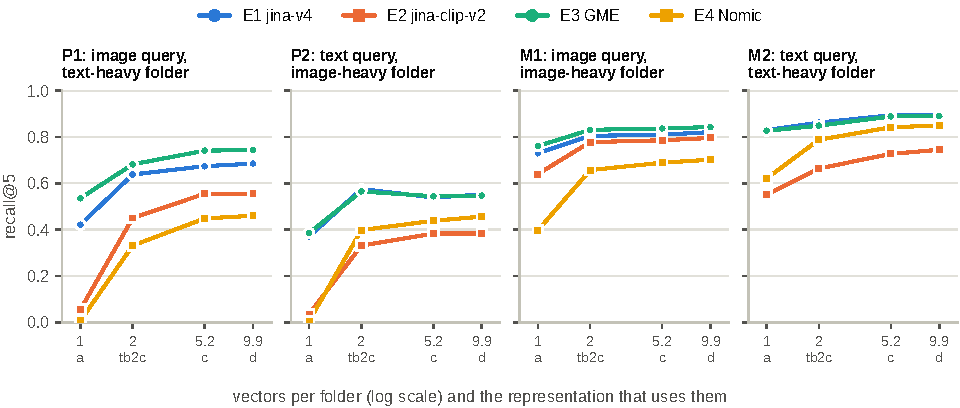
\includegraphics[width=\textwidth]{figures/fig_budget.pdf}
\caption{What each budget keeps: recall@5 on S11 by cell and encoder for the pooled centroid \rep{a} (one vector), two blind centered clusters \rep{tb2c}, per-modality $k$-means \rep{c} and every file \rep{d} (Table~\ref{tab:cells}). Circles are vision-language embedders and squares dual towers. Most of what the flat walk gains over one vector is already there at \rep{c}.}
\label{fig:budget}
\end{figure}

\paragraph{Five per-modality representatives stay close to the flat walk under all four encoders.} \rep{c}, per-modality $k$-means with at most three representatives per label, uses 5.2 vectors per folder on S11, a little over half the files. Its point estimates are within 0.018 of the flat walk \rep{d} over all queries and in the four cells under all four encoders (Table~\ref{tab:cells} and Figure~\ref{fig:budget}), and within 0.013 on S3 and S5. The rule pre-registered under E3 and E4, that no interval lie entirely below $-0.02$, is not a test of non-inferiority. Read as one, with the lower bound at or above $-0.02$, \rep{c} passes over all queries under all four encoders, with the lowest bound at $-0.015$, and in every cell under E3. One cell falls just below under E1 (M1, $-0.021$) and one under E2 (M2, $-0.025$), and three under E4, down to $-0.024$ (session 25). On the 77 percent of S11 queries whose folder \rep{c} strictly compresses, \rep{c} minus \rep{d} is $-0.006$ \ci{-0.011}{-0.002} over all queries under E1 (post hoc). Its centered form \rep{cc} is above \rep{d} in the minority cells under E1 and E2, and in P2 under E3 and E4. Two blind clusters pass their pre-registered margin under E1, by the rule and with point losses of 0.03 to 0.04 in two cells, and fall short of it under the other three encoders, among them E3, a vision-language embedder like E1.

\paragraph{Budgets from one to eight centroids.} Session 27 varied the budget on the confirmation set under all four encoders, with its reading registered before the new rows were computed (Figure~\ref{fig:budgetsweep}). The set had been read before and some rows, among them \rep{c}, were known, so we mark the reading post hoc. Three families were scored, uncentered and centered. The labelled family keeps $\min(k, n_m)$ centroids per label for $k$ from 1 to 5, so that $k = 3$ is \rep{c}. The blind family keeps $K$ centroids over the whole folder for $K$ in 2, 3, 4, 5, 6 and 8, and a third family keeps as many blind centroids in each folder as the labelled one does. A budget qualifies under an encoder when the lower end of the interval of its difference from \rep{d} is at or above $-0.02$ over all queries and in each of the four cells. Four per label, 6.02 vectors per folder, is the smallest labelled budget that qualifies under all four encoders, uncentered or centered. Three per label qualifies uncentered under E3 only. As the reading of session 25 found, it falls just below the margin in M1 under E1 ($-0.021$), in M2 under E2 ($-0.025$) and in three cells under E4, down to $-0.024$. Centered, three per label qualifies under E1, E2 and E3. One and two per label qualify under no encoder. Uncentered blind centroids qualify under E4 at no $K$ up to eight. Centered, they need eight (6.13 vectors per folder) under all four encoders and four under E1. With about six vectors per folder the centered rows reach the uncentered flat walk \rep{d} over all queries under every encoder. Four centered centroids per label minus \rep{d} is $+0.010$ \ci{+0.006}{+0.014} under E1, $+0.007$ \ci{+0.003}{+0.011} under E2, $+0.003$ \ci{-0.000}{+0.005} under E3 and $+0.004$ \ci{+0.000}{+0.008} under E4. On the second GitHub draw, read under E1 without a verdict, no budget qualifies in the minority cells P1s and P2s, where the intervals resample owners and are wider. There four per label minus \rep{d} is $-0.015$ \ci{-0.031}{-0.002} and $-0.018$ \ci{-0.033}{-0.005}. Section~\ref{sec:discussion} reads what the labels buy at the same number of vectors.

\begin{figure}[tp]
\centering
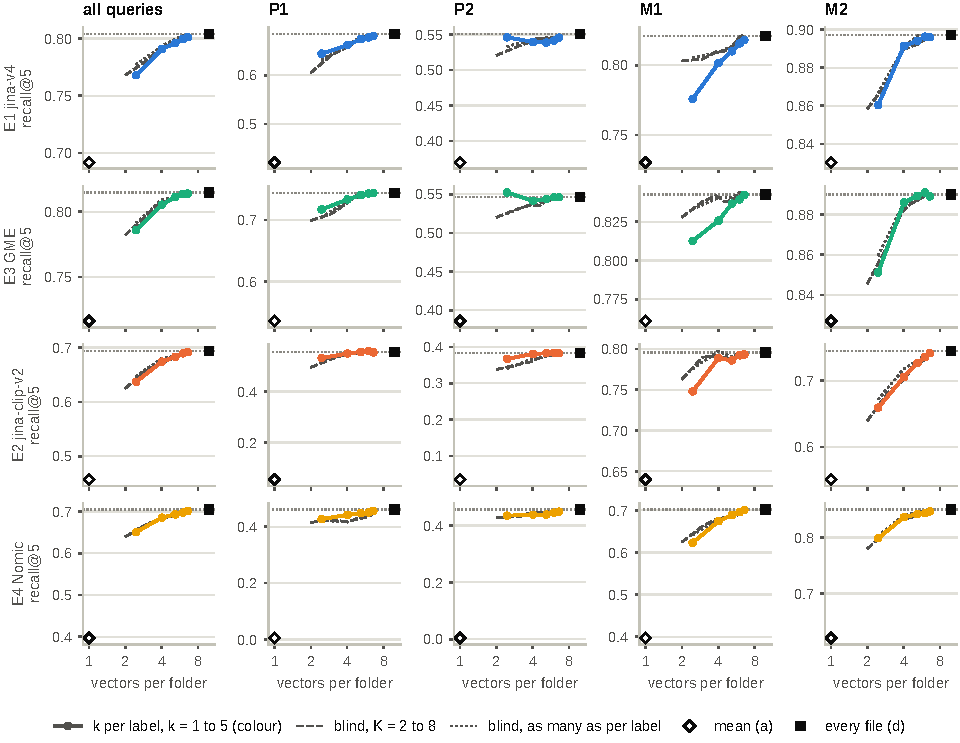
\includegraphics[width=\textwidth]{figures/fig_budgetsweep.pdf}
\caption{Budgets from one to eight centroids (session 27, confirmation set, post hoc, uncentered rows): recall@5 against the mean number of vectors per folder, by encoder (rows) and cell (columns). Coloured lines with dots keep $k$ centroids per label for $k$ from 1 to 5, the third dot being \rep{c}. Dashed lines keep $K$ blind centroids for $K$ from 2 to 8, and dotted lines as many blind centroids as the labelled row keeps in each folder. The open diamond is the pooled centroid \rep{a}, and the filled square, with its level as a dotted line, is every file \rep{d}.}
\label{fig:budgetsweep}
\end{figure}

\paragraph{The budget in bytes.} A metadata field counts bytes. In float32 the representatives of \rep{c} take 42,594, 21,297, 31,945 and 15,973 bytes per folder on average under E1 to E4. Session 20 stored every vector of \rep{a}, \rep{c} and \rep{d} in five formats and scored the S11 evaluation queries again under the four encoders. The formats are float32, float16, one byte per dimension (int8: the vector divided by its largest absolute entry, multiplied by 127 and rounded), four bits (int4: the same with 7) and one bit (bin: the sign). A stored vector is decoded and normalised before scoring, and the query stays in float32, since it is embedded at search time. Nothing is fitted. \citet{shakir2024quantization} describe such quantisation of finished embeddings. They threshold at zero for one bit, as we do, and map each dimension's range to one byte with a calibration set, where we scale each vector by its own largest entry. Binary codes can also be learned \citep{yamada2021bpr}. In float32 the \rep{a}, \rep{c} and \rep{d} rows reproduce the ranks behind Table~\ref{tab:cells} query for query under all four encoders.

Three hypotheses were fixed before the run. H20a applies the rule of H15b at one byte per dimension: no interval of \rep{c} at one byte minus \rep{d} in float32 may lie entirely below $-0.02$ over all queries or in P1, P2, M1 or M2. It survived under all four encoders. One byte per dimension costs nothing measurable. Against \rep{c} in float32 the difference is within 0.001 in every cell under every encoder. \rep{c} then takes 10,648, 5,324, 7,986 and 3,993 bytes per folder on average under E1 to E4, and at most 28,672. H20b applies the same rule at one bit per dimension. It survived under E1 and E3 and died under the two dual towers, under E2 in M2 ($-0.033$ \ci{-0.041}{-0.025}) and under E4 over all queries ($-0.057$ \ci{-0.062}{-0.051}), in P1 and in M1. Under E4 one bit costs every stored vector. Over all queries it changes \rep{c} by $-0.045$ and the flat walk by $-0.048$ \ci{-0.053}{-0.044} against their float32 forms, and at one bit \rep{c} is 0.009 below the flat walk. H20c required \rep{c} at one bit per dimension to beat the pooled centroid in float32 in P1 and in P2. It survived under all four encoders, with differences from $+0.172$ to $+0.503$. At one bit \rep{c} takes 1,331, 666, 998 and 499 bytes per folder on average under E1 to E4, against 8,192, 4,096, 6,144 and 3,072 for the single float32 vector of \rep{a}.

\begin{table}[t]
\centering\small
\caption{\rep{c} in a metadata field of fixed size (session 20, S11). For each budget per folder, the most precise format in which every folder's \rep{c} fits and its recall@5 over all queries, in P1 and in P2. The formats f32 and f16 are single and half precision, int8 is one byte per dimension, int4 four bits and bin one bit. None means that no format fits. The last two rows give \rep{c} and \rep{a} in float32 without a budget. Vision-language embedders above, dual towers below.}
\label{tab:bytes}
\begin{tabular}{llrrrlrrr}
\toprule
& \multicolumn{4}{c}{E1 jina-embeddings-v4} & \multicolumn{4}{c}{E3 gme-Qwen2-VL-2B} \\
\cmidrule(lr){2-5}\cmidrule(lr){6-9}
Budget & format & all & P1 & P2 & format & all & P1 & P2 \\
\midrule
2 KiB & none & & & & none & & & \\
4 KiB & bin & 0.796 & 0.676 & 0.543 & bin & 0.810 & 0.743 & 0.558 \\
8 KiB & bin & 0.796 & 0.676 & 0.543 & bin & 0.810 & 0.743 & 0.558 \\
16 KiB & int4 & 0.794 & 0.673 & 0.540 & int4 & 0.807 & 0.742 & 0.547 \\
64 KiB & f16 & 0.796 & 0.674 & 0.539 & f16 & 0.811 & 0.741 & 0.544 \\
\rep{c}, no budget & f32 & 0.796 & 0.674 & 0.539 & f32 & 0.811 & 0.741 & 0.544 \\
\rep{a}, no budget & f32 & 0.692 & 0.421 & 0.370 & f32 & 0.716 & 0.536 & 0.386 \\
\midrule
& \multicolumn{4}{c}{E2 jina-clip-v2} & \multicolumn{4}{c}{E4 Nomic Embed v1.5} \\
\cmidrule(lr){2-5}\cmidrule(lr){6-9}
Budget & format & all & P1 & P2 & format & all & P1 & P2 \\
\midrule
2 KiB & bin & 0.675 & 0.558 & 0.376 & bin & 0.648 & 0.377 & 0.431 \\
4 KiB & bin & 0.675 & 0.558 & 0.376 & bin & 0.648 & 0.377 & 0.431 \\
8 KiB & int4 & 0.676 & 0.554 & 0.379 & int4 & 0.692 & 0.443 & 0.441 \\
16 KiB & int8 & 0.683 & 0.554 & 0.382 & int8 & 0.693 & 0.447 & 0.438 \\
64 KiB & f32 & 0.683 & 0.555 & 0.383 & f32 & 0.693 & 0.448 & 0.438 \\
\rep{c}, no budget & f32 & 0.683 & 0.555 & 0.383 & f32 & 0.693 & 0.448 & 0.438 \\
\rep{a}, no budget & f32 & 0.457 & 0.055 & 0.035 & f32 & 0.397 & 0.006 & 0.005 \\
\bottomrule
\end{tabular}
\end{table}

Table~\ref{tab:bytes} reads the same rows by budget. The brief fixed five budgets per folder, 2, 4, 8, 16 and 64 KiB. It tied 2, 4 and 64 KiB to real limits, and limits near 8 and 16 KiB were looked up after the run. Amazon S3 limits the user-defined metadata of an object to 2 KB, and it also offers a store of another kind, annotations of up to 1 MB each \citep{aws2026s3metadata}. On ext4 the block that holds a file's attributes outside its inode is at most 4,096 bytes, and APFS keeps a value inside the file-system record up to 3,804 bytes \citep{linux2026xattr,e2fsprogs2025ext4,apple2020apfs}. Google Cloud Storage allows 8 KiB of custom metadata per object \citep{google2026gcsquotas}. Btrfs limits an attribute with its name to the node size, 16 KiB by default, and 64 KiB is the ceiling of one attribute value on Linux \citep{linux2026xattr}. At 8 KiB every folder's \rep{c} fits under every encoder, at one bit per dimension under E1 and E3 and at four bits under E2 and E4. In those formats it is at most 0.012 below \rep{c} in float32 in any of the five cells and 0.007 below over all queries, both under E2. The rule of H15b was registered for one byte and for one bit. Read as a secondary at four bits, it passes under E4 and fails under E2, at $-0.030$ \ci{-0.038}{-0.022} in M2, so at 8 KiB \rep{c} passes it under E1, E3 and E4. At 16 KiB every folder's \rep{c} fits at four bits under E1 and E3 and at one byte under E2 and E4, and by the same reading no interval lies entirely below $-0.02$ under any encoder. At 64 KiB it fits in float16 or float32. The flat walk has no fixed size. It grows with the folder, to 491,520 bytes in float32 under E1 for a folder of 60 files, and at 8 KiB it fits every folder only under E2 and E4 at one bit. \rep{c} is bounded by three representatives per modality label and holds at most 14 on S11. These sizes count the stored vectors alone. On most of the systems above the limit also covers the attribute's name, and on several all the attributes of one file or object together.

\paragraph{What to keep in two kilobytes.} Session 20 fixed the summary and varied its format. Session 21 fixed the bytes and asked which summary to put in them, on the cached vectors of both sources. At 2 KiB, the user-metadata allowance of Amazon S3 and half an ext4 block, a folder's metadata holds eight one-bit vectors under E1, or its mean at one byte per dimension. A folder that fits whole keeps every file at one bit. Otherwise the policies differ in what the eight slots hold. \emph{sample} keeps eight of the folder's files, dealt to the kinds present and chosen by a hash of each file's path. \emph{usample} keeps the eight files of smallest hash with the kinds ignored, a bottom-$k$ sketch \citep{cohen2007bottomk} that a parent can compute exactly from its children's. \emph{kmeans} keeps eight spherical $k$-means centroids. Medoids, farthest-first files and one mean per kind are matched baselines at the same bytes. Three tests were fixed on S19 under E1, read on 98.33 percent intervals, on the queries whose folder does not fit whole (3,333 of the 7,372, and 310 of the 581 minority queries). On the minority queries, sample minus the mean is $+0.269$ \ci{+0.158}{+0.384} (H21a) and sample minus the uniform sample $+0.116$ \ci{+0.054}{+0.187} (H21c), both from 70 owners and so inconclusive by the owner minimum. Over all queries, sample minus kmeans is $-0.042$ \ci{-0.060}{-0.026} from 207 owners, so the sample is inferior to the centroids at the registered margin (H21b).
Session 24 read the three tests again on the second GitHub draw, with 146 owners in the minority cell and 365 over all queries. Sample minus the mean is $+0.252$ \ci{+0.181}{+0.327}, confirmed, sample minus kmeans $-0.052$ \ci{-0.067}{-0.038}, inferior, and sample minus the uniform sample $+0.097$ \ci{+0.054}{+0.145}, so the kinds matter. For a test whose first-draw cell missed the owner minimum, the brief of session 24 fixed the pooled reading as the one the paper takes. Pooled over both draws, H21a is confirmed at $+0.258$ \ci{+0.198}{+0.321} and H21c reads that the kinds matter, at $+0.103$ \ci{+0.067}{+0.142}. H21b is inferior on both draws and pooled ($-0.048$ \ci{-0.060}{-0.037}).
The same signs hold on Zenodo and under the other encoders (Table~\ref{tab:twokib}). The table prints 95 percent intervals for every row. The registered readings above are on 98.33 percent intervals, which are wider, so the same statistic carries two intervals in this section. On the minority queries of S19 under E1, eight one-bit vectors chosen with the kinds or the clusters in view reach the level of every file in float32. Their owner-weighted recall@5 is 0.624 for sample and 0.626 for kmeans, against 0.628 for every file in float32 and 0.423 for the mean at one byte per dimension. On the folders that do not fit, clustering buys 0.03 to 0.08 of recall@5 over the sample. A summary made of the files' own vectors, which a directory can keep up to date without clustering, pays that much for it.

\begin{table}[t]
\centering\small
\caption{What to keep in 2 KiB of folder metadata (session 21): recall@5 differences between summaries of equal size, on the queries whose folder does not fit whole. \emph{sample}: files at one bit dealt to the kinds present; \emph{usample}: the files of smallest hash, kinds ignored; \emph{kmeans}: centroids at one bit; \emph{mean}: one vector in the most precise format that fits. 95 percent intervals, from 10,000 resamples of owners on the GitHub draws (owner-weighted) and from 1,000 resamples of directories on S11 (query-weighted). The registered tests are the S19 rows under E1 (Section~\ref{sec:remedy}).}
\label{tab:twokib}
\begin{tabular}{llll}
\toprule
Set, encoder & sample $-$ mean, minority & sample $-$ kmeans, all & sample $-$ usample, minority \\
\midrule
S19, E1 & $+0.269$ \ci{+0.178}{+0.365} & $-0.042$ \ci{-0.057}{-0.029} & $+0.116$ \ci{+0.064}{+0.173} \\
S19, E4 & $+0.444$ \ci{+0.231}{+0.671} & $-0.032$ \ci{-0.066}{-0.008} & $+0.067$ \ci{+0.000}{+0.167} \\
S19, E2 & $+0.453$ \ci{+0.292}{+0.616} & $-0.033$ \ci{-0.058}{-0.013} & $+0.049$ \ci{-0.026}{+0.133} \\
S24, E1 & $+0.252$ \ci{+0.193}{+0.312} & $-0.052$ \ci{-0.064}{-0.040} & $+0.097$ \ci{+0.061}{+0.136} \\
S11, E1 & $+0.308$ \ci{+0.266}{+0.354} & $-0.078$ \ci{-0.090}{-0.065} & $+0.107$ \ci{+0.086}{+0.131} \\
S11, E3 & $+0.287$ \ci{+0.235}{+0.340} & $-0.059$ \ci{-0.071}{-0.047} & $+0.064$ \ci{+0.048}{+0.083} \\
S11, E2 & $+0.704$ \ci{+0.662}{+0.746} & $-0.053$ \ci{-0.064}{-0.043} & $+0.078$ \ci{+0.059}{+0.098} \\
S11, E4 & $+0.706$ \ci{+0.647}{+0.756} & $-0.044$ \ci{-0.053}{-0.034} & $+0.055$ \ci{+0.033}{+0.080} \\
\bottomrule
\end{tabular}
\end{table}

\paragraph{Written to a file system.} Session 22 wrote summaries of 2,048, 4,000 and 8,192 bytes to ext4 with 4 KiB blocks, for 300 repository trees from the list of session 19 (9,934 directories, 50,906 files), and counted the blocks a reader fetches after a fresh mount. No hypothesis was read on it. On a cold descent with readahead off, an attribute of the directory costs 1.20 blocks per summary at 2,048 and at 4,000 bytes, a sidecar file in the directory 2.04, and one packed index per tree 0.82 and 1.33. Reading the one-bit vectors of a directory's files instead costs 5.61 blocks a directory on default ext4, where an attribute of 256 bytes does not fit an inode of 256 bytes, and 2.04 with inodes of 1,024 bytes. A summary of 8,192 bytes is an ext4 attribute only with the ea\_inode feature, at 2.30 blocks to read and 23.9 blocks written to replace it, against 7.0 written at 2,048 or 4,000 bytes. With the kernel's readahead as shipped, the packed index reads more than the attribute at every size. A directory's attribute survives \texttt{cp -a}, a tar archive made with extended attributes and a move within the file system. It is lost by a plain \texttt{cp -r}, by tar with its default options and by git, which stores no extended attribute. These are block counts on one kernel and one file system. Times were not measured.

\section{Walking a repository tree}
\label{sec:tree}

The idea this study started from is a summary on each folder that says what the folder holds, so that a reader can pick the directory to walk down whatever the folder is called. Session 23 built that walk on whole repository trees. From the pool of session 19, read in an order of its own, it took a repository whole when at least eight of its directories hold a kept file, one of them at depth two or more, with 40 to 300 kept files, at least five of them images and five not. The harvest stopped at its limit of 33,000 files with 261 trees, 11.2 percent of the 2,328 repositories read, and 33,092 files in 8,587 directories. Every directory has a summary of its subtree, and a directory with files also has one of its own files. The held-out query is removed from every summary that held it. The reader starts at the root. At each directory it scores staying by the directory's own summary and each child by the child's subtree summary, takes the best and stops when staying wins. A walk succeeds when it stops in the query's directory. The flat reader reads the own summary of every directory of the repository and takes the best. The summaries are those of Section~\ref{sec:remedy} at 2 KiB, with one difference. A summary that a parent computes from its children's has to merge exactly, so the sample here keeps a fixed share of its slots per kind (\emph{fsample}), and a kind with fewer files leaves its slots empty. The uniform sample merges exactly as it is. The minority cell holds the queries of the repository's smaller input group whose directory keeps a sibling of their group, 2,844 of the 20,814 queries, from 208 of the 259 owners.

Three tests were fixed at 2 KiB under E1, before any tree was read (Table~\ref{tab:tree}). The per-kind sample walks to the minority files $+0.024$ \ci{-0.022}{+0.073} more often than the mean, so H23a is inconclusive, and at the registered size a per-kind summary did not measurably help the walk. Among summaries that merge exactly, the kinds matter. fsample beats the uniform sample on the minority files by $+0.064$ \ci{+0.028}{+0.104} (H23b). The walk reads 0.39 as many summaries as the flat reader (12.7 against 32.7 per query) and finds the target 0.069 \ci{0.054}{0.086} less often, so H23c reads inferior. At 2 KiB the summaries serve a flat read of a tree better than a descent.

Over all queries the mean is the best summary for the walk at 2 KiB, at 0.630 against 0.528 for fsample, and it stays the best at 8 KiB, against 0.605 for fsample. fsample stores 2.86 vectors in an own-files summary and 3.86 in a subtree summary on average, against eight slots, and the subtrees a walk compares near the root hold far more files than that. A plausible reading is that a few sampled files cover a large subtree's majority worse than its mean does. At 8 KiB, a secondary without a reading, the per-kind sample walks to the minority files $+0.067$ \ci{+0.031}{+0.103} more often than the mean, and the walk comes within 0.017 of the flat read. Every vector summary beats a reader of file names, which reaches 0.477 over all queries, by $+0.050$ \ci{+0.026}{+0.074} for fsample at 2 KiB and $+0.127$ at 8 KiB. For the samples, walk success falls with the depth of the target, from 0.698 at the root to 0.439 at depth three or more for fsample, while the mean holds at 0.574 at depth three or more. A walk compounds its errors over the levels.

\begin{table}[t]
\centering\small
\caption{Walking whole repository trees (session 23, 261 trees, E1). Owner-weighted success of a walk that stops in the query's directory and of a flat read that ranks every directory's own summary, over all 20,814 queries and the 2,844 minority queries, and the summaries a walk reads per query (Reads; the flat read reads 32.7). \emph{fsample} keeps a fixed share of its one-bit slots per kind and merges exactly up the tree; \emph{usample} is the bottom-$k$ sample by hash; \emph{sample} refills empty slots and does not merge exactly. The registered tests are at 2 KiB.}
\label{tab:tree}
\setlength{\tabcolsep}{5pt}
\begin{tabular}{llrrrrr}
\toprule
Budget & Summary & Walk, all & Walk, minority & Flat, all & Flat, minority & Reads \\
\midrule
2 KiB & mean & 0.630 & 0.686 & 0.671 & 0.782 & 14.1 \\
 & usample & 0.542 & 0.646 & 0.599 & 0.745 & 13.0 \\
 & fsample & 0.528 & 0.710 & 0.597 & 0.745 & 12.7 \\
 & sample & 0.537 & 0.723 & 0.599 & 0.746 & 12.9 \\
8 KiB & mean & 0.630 & 0.686 & 0.671 & 0.782 & 14.1 \\
 & usample & 0.614 & 0.731 & 0.622 & 0.753 & 14.4 \\
 & fsample & 0.605 & 0.753 & 0.622 & 0.753 & 14.2 \\
 & sample & 0.613 & 0.753 & 0.622 & 0.753 & 14.3 \\
none & every file at one bit & 0.625 & 0.753 & 0.625 & 0.753 & 14.8 \\
 & file names & 0.477 & 0.649 & 0.478 & 0.655 & 14.7 \\
 & chance & 0.069 & 0.092 & 0.047 & 0.049 & \\
\bottomrule
\end{tabular}
\end{table}

\section{Knowing the target type}
\label{sec:type}

A searcher often knows the kind of file wanted, an image or a PDF, and a file system knows each file's kind for free. Session 16 asked, pre-registered, whether a folder's type composition helps then. The composition is a few counts and fits beside the vectors in the folder's metadata. The kind is image, pdf (text or scanned), text, table or other, and a folder's composition counts its files of each kind, the query file included, since the stored folder holds it. Three uses were tested on the S11 evaluation queries under all four encoders, on top of \rep{a}, \rep{c} and \rep{d}. A filter ranks only the folders that hold the query's kind. A prior adds $\tau$ times the logarithm of the kind's share in the folder to the score, with $\tau$ chosen on the calibration queries. Type-only groups score a folder by its representatives of the query's kind alone, and for \rep{a} that is one pooled vector per kind (2.42 per folder). Type-only groups are compared on the 15,448 queries whose folder keeps another file of their kind, since under leave-one-out the others have nothing to match.

The filter changes little here. It adds 0.004 to 0.008 recall@5 over all queries. Image queries gain nothing, since 96.8 percent of the folders hold an image, and the rarer kinds gain more, up to 0.083 for scanned PDFs under E1 with \rep{a}. With the filter the pooled centroid still loses the minority, by $+0.153$ to $+0.500$ in P1 and P2 across the four encoders, every interval above zero (H16a). On the queries that have another file of their kind in the folder, one pooled vector per kind recovers most of the pooled centroid's loss, by $+0.206$ to $+0.607$ in P1 against the filtered centroid. It falls short of per-type $k$-means representatives in the majority cells under every encoder, by 0.035 to 0.065 in M1 and 0.035 to 0.068 in M2, so the hypothesis that one vector per type keeps them died (H16b). Within one kind a folder can hold many files, and one mean is too coarse for them. Restricting \rep{c} to the query's kind costs 0.002 to 0.013 recall@5 against the filter over the same queries, and up to 0.034 in P1. At the weight the calibration queries chose, 0.001 or 0.002, the prior changes recall@5 by at most 0.002 over all queries and by at most 0.010 in any of the five cells. H16c needed it to lower both minority cells, and under each encoder at least one of the two intervals does not lie below zero, so H16c died. Larger weights lower the minority cells and recall overall. Of the majority cells only M1 gains, by 0.009 at most, and M2 falls. Under E1 at $\tau = 0.05$, P1 falls from 0.674 to 0.584 while M1 rises from 0.810 to 0.816. A tree of single-type folders would gain more from the filter, and this corpus cannot show that.

\section{A folder layer as an index}
\label{sec:systems}

A folder layer promises a cheaper search. It ranks folders by a few vectors and then searches the files inside the top few. We measured the promise on S5 against the exhaustive flat walk and against a flat HNSW index \citep{malkov2020hnsw} over all 27,243 file vectors (hnswlib 0.8.0, $M = 16$, ef\_construction 200, one thread, 2,000 timed queries, best of three passes). In the two-stage form, stage one ranks directories by representation $x$ and stage two ranks the files of the top $k = 10$ directories exactly. Hit@10 is whether a sibling of the query is in the top ten files.

With \rep{c} as stage one, the two-stage search is within 0.001 hit@10 of the exact flat walk \rep{d} ($-0.001$ \ci{-0.003}{+0.001}), so H5 survives its recall clause. It scores 0.55 of the vectors, though, because \rep{c} keeps up to three representatives per label whatever the group's size and the set has 9.7 embedded files per directory, so H5's cost clause fails. A budget that scales with group size, $k = \min(3, \lceil n_m / 4 \rceil)$, scores 0.355 of the vectors and loses 0.007 hit@10 (H6 dead on cost, by 0.005). Against flat HNSW the layer buys nothing. We put HNSW over the \rep{c} representatives as stage one and compared it with the flat index at the pre-registered matched setting, the smallest ef\_search at which the flat index is not faster than the two-stage search (128, at 462 $\mu$s against 345 $\mu$s). Hit@10 differs by $+0.0006$ \ci{-0.0012}{+0.0023}, so H7 is dead. Timing the same indexes a second time moved the matched setting to ef\_search 192 and the difference to $+0.0003$ \ci{-0.0015}{+0.0020}. The two-stage index is 1.53 times the flat one in storage. On the same one-thread build, flat HNSW at ef\_search 64 answers in 200 $\mu$s at recall@10 0.994 against exact search. At this scale (tens of thousands of in-memory vectors, one thread, frozen embeddings) every indexed method answers in under a millisecond. The exhaustive walk takes 5.2 ms and exact two-stage search with \rep{c} 2.9 ms. At this scale the folder layer matters only through its representation. A flat index holds every file's vector in one place, which the metadata setting does not have, so it stands beside the flat walk as a reference for that setting. Partitioned designs win at billion scale with posting lists on disk \citep{chen2021spann}, and directory scopes are a filtering problem with indexes of their own \citep{wang2026directoryaware,patel2024acorn}. Our result does not reach there. It does not need to, because the loss of Section~\ref{sec:loss} is present whenever a folder vector is scored at all, whether the folder is a routing unit, a memory or a search result in its own right.

\section{Discussion}
\label{sec:discussion}

\paragraph{The rule for a router or an agent's memory.} Consider a system that keeps one vector per folder, collection or source and routes queries on it, such as a source router for retrieval-augmented generation \citep{dhasade2026ragroute}, an agent's directory-shaped memory or a folder-level file search. The results support one rule for it. Where a folder does not mix images with other files, keep the mean. Where it does, keep a few representatives per kind. A file system tells the two apart by file type without embedding anything. On GitHub directories, 4 to 5 percent of eligible ones mix media. On the others a few representatives lose a little to the mean, and keeping them only for the mixed folders keeps most of the minority gain and is level with the mean over all directories (Section~\ref{sec:github}, post hoc). It was not shown to beat representatives for every folder.

\paragraph{What the mean loses where a folder mixes.} On our Zenodo folders, recall@5 on minority-modality file queries is 16 to 25 points lower with the pooled vector than with per-modality representatives under two vision-language embedders from different vendors, and 35 to 50 points lower under two CLIP-family dual towers. On GitHub directories it is about 20 points lower under the first of those embedders, on two draws. On queries that a model wrote as a simulated searcher from what a person sees of a folder, it is 14 points lower for pictures in text-heavy folders and 42 for documents in image-heavy ones under the first embedder. Under E2 the picture cell shows no loss (Section~\ref{sec:searcher}). With fewer collections competing the loss is smaller, 0.01 to 0.05 among 10 and 0.11 to 0.16 among 100 (post hoc), so a router that chooses among a few sources loses little of it.

\paragraph{How many vectors, and in how many bytes.} The fix is an old one \citep{weston2013maxmf,pal2020pinnersage}, a few representatives per kind scored by the maximum. On the confirmation set four per label, about six vectors per folder, were not inferior to file-level search over all file queries and in every cell under all four encoders (Section~\ref{sec:remedy}, post hoc). Three per label, about five vectors, met the same margin over all queries under all four encoders and in every cell under E3. At three per label a folder stores a little over half as many vectors as it has files. At one byte per dimension that is 3,993 to 10,648 bytes per folder on average by encoder, and every S11 folder fits in 8 KiB at one or four bits per dimension, at a cost of at most 0.012 in any cell. Written to ext4 as an extended attribute of the directory, a summary of 2,048 or 4,000 bytes costs 1.2 blocks per directory read on a cold descent, and one of 8,192 bytes needs the ea\_inode feature and 2.3 blocks. On whole repository trees at 2 KiB, the summaries guide a flat read better than a descent, and the mean routes a walk best over all queries. A per-kind sample beats it on the minority files only at 8 KiB (Section~\ref{sec:tree}). A summary written by a language model, which RAPTOR uses for clusters of text chunks and OpenViking for directories, does not replace them. Added to them it gains a little on whole-folder text queries. Alone it does no better than the pooled vector at finding a minority image from its description (Section~\ref{sec:abstracts}). Per-modality mean-centering, the single-item fix \citep{li2025grclip}, is worth doing on the file side, where over all file queries it helps the pooled vector, the per-modality representatives and file-level search under all four encoders. It does not replace the representatives. Under E3 it recovers 8 percent of the loss on image queries in text-heavy folders. Applied to a text query with the file-side mean, its effect depends on the encoder. Over all title queries it does nothing under E1, hurts under E2 and helps under E3 and E4 (Section~\ref{sec:nlq}).

\paragraph{The folder is two clusters, and modality is the usual reason.} The dilution control suggests, on ten hosts, that a pooled vector loses any foreign minority, of the folder's modality or not, and that the modality gap adds to the loss. Blind clustering finds the modality partition because, in this corpus, modality is where the within-folder structure is. In a corpus whose folders split along topic or language instead, we would expect label-blind clusters to help and labelled ones not to. In the control the labelled pair could not see a same-modality guest and the blind pair could (Section~\ref{sec:dilution}). We have not measured such a corpus. We present per-label representatives as the practical form. A file system knows a file's type for free, and four per label met the margin against file-level search under all four encoders, where blind centroids needed eight with centering and never met it without centering under E4 (Section~\ref{sec:remedy}). The label does not replace the clustering. \rep{c} still runs $k$-means inside each label, and what the type buys is the split of the budget across the groups. Session 27 measured what that split is worth with the same number of vectors in every folder. At one per label, uncentered, the labels move recall from the majority image files to the minority files under E1 to E3. They gain $+0.013$, $+0.007$ and $+0.013$ in P1 and $+0.013$, $+0.027$ and $+0.027$ in P2, and they lose $0.029$, $0.028$ and $0.020$ in M1, while over all queries the blind split is level or ahead. Under E4 the gain at one per label is $+0.004$ in P1, against $0.018$ lost in M1. From three per label up the two are within 0.015 of each other in every cell under all four encoders, and over all queries the labels are at most 0.007 behind. Under E4, uncentered, the labels stay ahead in P1 at every count by the point estimate, by $+0.014$ \ci{+0.000}{+0.028} at three per label and $+0.014$ \ci{+0.005}{+0.024} at five. There blind centroids at the labelled count never meet the margin against file-level search, while four per label do. At equal bytes under E1 the labels added nothing, on the main set (H9c) and at 2 KiB on S11, where per-label centroids minus blind centroids is $-0.002$ \ci{-0.004}{-0.000} over all queries (session 25, post hoc). From three per label up, blind $k$-means at the same count is about as good a default as the labels, except under E4 without centering.

\paragraph{Limitations.} \emph{Two sources.} The Zenodo folders are deposits by researchers under CC0 or CC-BY of 3 to 60 files, whose images are mostly figures. The three later Zenodo draws are disjoint but come from one search of one repository, and 527 of the 2,597 S11 records share their first creator with a record of S5. The GitHub directories come from public repositories with at least five stars and a permissive licence, and they are read under E1 alone on the second draw and under E1, E4 and E2 on the first. Personal working directories, mailboxes and agent memories were not measured. Within S11 the records are not independent either. Some creators deposited many records, and about 47 effective creator families stand behind the 2,146 text queries in image-heavy folders. Section~\ref{sec:validity} resamples creators and sets aside the queries whose file names give their folder away, and the verdicts re-read there do not move. The other Zenodo intervals, among them those of the hypotheses of sessions 3, 5 to 10, 16 and 20, resample directories only. The GitHub tests of sessions 19, 21 and 24 resample owners. The Zenodo pool was selected for records that hold both an image type and a document type, and the GitHub scored sets over-sample mixed directories, so the study measures how much a mixed folder loses. How common mixed folders are was counted only among the eligible directories of the GitHub repositories read, 4.2 percent on the first draw and 5.0 on the second. The natural-mix estimates reweight strata that take at most two directories per stratum and repository. The mixed-only policy was tested on draws the study had already read. \emph{Ground truth.} Relevance is structural. The one relevant folder of a query file is its own, and a record's title or description is relevant to that record only. This measures whether a folder vector represents its files. It does not measure topical relevance across folders, and the queries of Section~\ref{sec:nlq} are the depositor's own words, which may also occur inside the record's files. No person wrote queries for this study. The searcher queries of Section~\ref{sec:searcher} and the image descriptions of Section~\ref{sec:abstracts} were written by models, and the commit subjects of Section~\ref{sec:github} by the people who made a change, to describe it. The searcher queries cover 100 folders of one set, with their tests read under E1, and a model's queries may be more specific than a person's. \emph{Encoders.} There are four, from three vendors. The two vision-language embedders are both built on Qwen vision-language models (Qwen2.5-VL-3B and Qwen2-VL-2B), so they share a lineage, and the second was measured on the confirmation set only, under one calibration seed. The dual towers were measured on the confirmation set only, and the second under one seed. Both towers passed the pilot check weakly and are the two weakest encoders here, so their larger loss is partly the encoders and not only the wider gap. E4's tokenizer cut 14 of the 12,757 texts of the confirmation set at 8,192 tokens, so E4 read less of those texts than the other encoders did. The two input groups are images (with page renders of scanned PDFs) and extracted text. Audio and video were not included. \emph{Scale.} Each Zenodo set ranks 400 to 2,808 folders of ten to twelve files on average, as one flat set. The trees of Section~\ref{sec:tree} are 261 repositories admitted with 40 to 300 kept files, walked under E1 alone with held-out files as queries. Larger folders, deeper trees and more candidates were not measured, and the conclusion of Section~\ref{sec:systems} holds for tens of thousands of in-memory vectors only. \emph{The metadata setting.} The byte budgets of Section~\ref{sec:remedy} count stored vectors and nothing else. Summaries were written to one file system, ext4 on one kernel, as random bytes of the right sizes, and the blocks read were counted. Other file systems, a real summary maintained on writes, and the time to read a folder's attribute against listing and opening its files were not measured. The formats are plain rounding with no learned codebook and no calibration. Folders here hold at most 60 files, and larger ones, where the flat walk grows and \rep{c} does not, were not measured. \emph{The controls.} The dilution control rests on the ten hosts with guest queries of both kinds, its interval runs from 0.02 to 0.35, and its guests are topically foreign. It shows that a same-modality minority is lost too, and it does not apportion the natural loss between dilution and modality. Two vectors passed their pre-registered test under E1 by the margin rule, with point estimates outside the margin in two cells, and fell short under E2 to E4. They are not a budget the study supports. The budget was varied on the confirmation set, which earlier sessions had read, and on the second GitHub draw no budget of the sweep meets the margin in the minority cells, where the intervals resample owners (Section~\ref{sec:remedy}). Three $k$-means seeds were compared, on the confirmation set only. The margin rules of H9b, H11a, H14b, H15b, H20a and H20b kill a claim only when an interval lies entirely below $-0.02$. Passing one shows that no loss beyond the margin was detected, not that two rows are equivalent. The margins themselves, 0.02 for the flat walk, 0.05 as the smallest loss of interest on GitHub and 0.005 for the mixed-only policy, were fixed in the briefs without an argument from the setting. The non-inferiority readings on the Zenodo sets are query-weighted. \emph{What was not tried.} Names and vectors were fused with equal weights only. Trained pooling networks, corrections of the gap that retrain the encoder and late-interaction encoders were not measured. A folder's representative vectors were combined by their maximum cosine throughout. The only other combinations tried are the single inner product of the partitioned vector F4 and the prior of Section~\ref{sec:type}. The written abstracts of Section~\ref{sec:abstracts} come from one model and one set of prompts fixed in advance, and were embedded under E1 and E3 only. The single-vector result is a statement about the 40 vectors we scored on the main set under E1, and the query-side centering constant was not fitted on queries. \emph{The evaluation code.} The audit of this paper found one bug in it, which was corrected (Section~\ref{sec:remedy}). Sessions 9, 10, 13, 16, 18 and 20 re-ran earlier rows and required identical ranks, which guards against drift and not against an error common to all runs. A second implementation, written from a specification without the first one's code, gives identical ranks for \rep{a}, \rep{c} and \rep{d} under E1 (Section~\ref{sec:validity}). The other rows rest on the first implementation.

\paragraph{Reproducibility.} The repository holds the data manifests (Zenodo record identifiers, file paths, licences, hashes), the ground truth and the embedding and evaluation scripts. It also holds every session brief with its pre-registered hypothesis and every results file with full tables and the deviations of its session. The embedding caches rebuild from the manifests, and the model revisions are pinned.

\section{Conclusion}

Under the first embedder, on GitHub directories that do not mix media, which are most of them, the mean of a folder's embeddings did at least as well as a few representatives (post hoc). Where a folder mixes images and texts, its files form two clusters in a shared embedding space, and the mean sits between them and loses the folder's minority modality. On Zenodo record folders the loss is 0.16 to 0.25 recall@5 under two vision-language embedders and 0.35 to 0.50 under two CLIP-family dual towers, and on GitHub directories it is about 0.2 under the first embedder for files with a sibling of their kind. On image queries it holds at about half its size with creators weighted equally or on queries whose file names do not give the folder away, and at about a quarter with both. On queries that a model wrote as a simulated searcher it is 0.14 for pictures in text-heavy folders and 0.42 for documents in image-heavy ones under the first embedder. A few representatives per kind recover it, and none of the single vectors we tried, centering included, does so without giving up the majority. Four per label were not inferior to exhaustive file-level search at a margin of 0.02, over all queries and in every cell, under all four encoders on the confirmation set (post hoc). Three per label fit every folder's metadata in 8 KiB at a further cost of at most 0.012 in any cell. A folder abstract written by a vision-language model does not replace them. Keeping representatives only for the folders that mix, chosen by file type, was level with the mean over all GitHub directories at their natural mix under the first embedder (post hoc). It was not shown to beat representatives for every folder. Each registered hypothesis was tested against a criterion fixed in advance, the analyses added after review are marked post hoc, and the hypotheses that died or stayed inconclusive are reported beside the ones that survived.

\section*{Use of AI}

I used AI assistants (Claude, Anthropic; Gemini, Google) throughout this work, for writing, coding, analysis and review. The sessions of Section~\ref{sec:design} were working sessions in which I directed such an assistant, the second implementation of Section~\ref{sec:validity} was written by one, and ``agent'' in the text means such an assistant. The rounds of review that the text mentions were done by such assistants. Models also produced study materials. Qwen3-VL-8B-Instruct wrote the image captions and folder abstracts of Section~\ref{sec:abstracts}, and Pixtral-12B wrote the image descriptions used there as queries. Claude Opus 5.5 wrote the searcher queries of Section~\ref{sec:searcher}, as a simulated searcher that was told nothing about the study. No person wrote queries for this study. I conceived and directed the study and take full responsibility for its content.

\bibliographystyle{plainnat-nonote}
\bibliography{../reports/citations_verified}

\appendix
\section{Pre-registered hypotheses and verdicts}
\label{app:hyp}

Each hypothesis was fixed in the study brief before its test was run. From session 3 on the results files copy it verbatim. Intervals are 95 percent paired bootstrap over directories, 1,000 resamples, unless stated. In sessions 17 and 18, in H26d and in H27a to H27c they resample the records' first-creator families instead (Section~\ref{sec:validity}). On the GitHub draws and trees (sessions 19, 21, 23, 24 and 26) they resample owners 10,000 times, and the estimate is the mean over owners of the owner's mean. There a test with fewer than 100 owners is inconclusive, a loss is read as in Section~\ref{sec:github} (confirmed, present with the size open, below $+0.05$ or inconclusive), and the primary tests of a session are read on 98.33 percent intervals. Session 27 reads its two loss tests together, each on its 95 percent interval (Section~\ref{sec:searcher}).

\begin{description}
\item[Claim (session 2, S1).] A pooled centroid loses image queries in image-heavy directories and per-modality representations do not. Kill: \rep{b} and \rep{c} do not beat \rep{a} on image queries in both $[.5,.8)$ and $[.8,1]$ by more than the bootstrap interval. \textbf{Dead}: in $[.8,1]$ \rep{c} minus \rep{a} is $-0.001$ \ci{-0.020}{+0.016} and \rep{b} minus \rep{a} $-0.018$ \ci{-0.029}{-0.007}.
\item[H (session 3, S3).] A pooled centroid loses queries whose modality is the minority in their directory; per-modality $k$-reps recover them. Kill: the interval of \rep{c} minus \rep{a} does not exclude zero in both minority cells. \textbf{Survived}: $+0.179$ \ci{+0.115}{+0.251}, $+0.200$ \ci{+0.135}{+0.270}.
\item[H5 (session 5, S5).] Two-stage retrieval with \rep{c} at $k = 10$ loses at most 0.01 hit@10 against exact \rep{d} and scores at most half the vectors. Kill: the interval of the hit@10 difference lies entirely below $-0.01$. The cost clause was not part of the kill criterion. \textbf{Recall clause survived} ($-0.001$ \ci{-0.003}{+0.001}); \textbf{cost clause failed} (share 0.55).
\item[H6 (session 6, S5).] A size-scaled budget \rep{c4}, with $k = \min(3, \lceil n_m / 4 \rceil)$ representatives per label, loses at most 0.01 hit@10 and scores at most 0.35 of the vectors. \textbf{Dead on cost}: share 0.355; $-0.007$ \ci{-0.009}{-0.004}.
\item[H7 (session 7, S5).] HNSW over \rep{c} as stage one beats flat HNSW on hit@10 at the matched setting (the smallest ef\_search at which the flat index is not faster). \textbf{Dead}: $+0.0006$ \ci{-0.0012}{+0.0023}.
\item[H8 (session 8, S5).] The centered pooled centroid recovers more than half of \rep{c}'s gain over \rep{a} in both minority cells. \textbf{Dead}: $-0.002$ \ci{-0.023}{+0.018} and $-0.001$ \ci{-0.020}{+0.019}; 49 percent recovered.
\item[H9a (session 9, S5; re-run in session 13 after the ranking fix).] No single vector in the encoder's space (families F1, F2) selected on the calibration queries is within 0.02 of \rep{c} in both minority cells and both majority cells; dead if all four intervals of the selected configuration reach above $-0.02$. \textbf{Survived} on the corrected rows: centered pooling at $\alpha = 0.5$ is $-0.048$ \ci{-0.077}{-0.021} in P1 and $-0.047$ \ci{-0.061}{-0.036} in M2; CORAL at $\alpha = 0.75$ is $-0.086$ \ci{-0.110}{-0.059} in P2 and $-0.049$ \ci{-0.062}{-0.038} in M2. As first printed, with the bug, the same four cells read $-0.061$, $-0.058$, $-0.094$ and $-0.056$.
\item[H9b (session 9, S5).] The selected F3 or F4 configuration is within 0.02 of \rep{c} over all queries and in the four cells; dead if any interval lies entirely below $-0.02$. \textbf{Survived by the rule} for the selected F3 configuration, centered per-label centroids \rep{bc} at 2.55 vectors per folder (M1 $-0.023$ \ci{-0.039}{-0.008}); \textbf{dead} for its two-vector reading \rep{bc2} (M2 $-0.034$ \ci{-0.045}{-0.024}) and for the selected F4 configuration (P1 $-0.077$ \ci{-0.098}{-0.060}).
\item[H9c (session 9, S5).] \rep{c} beats label-blind $k$-means at its budget in both minority cells. \textbf{Dead}: $+0.000$ \ci{-0.005}{+0.006} and $+0.001$ \ci{-0.005}{+0.006}; at that budget the blind clusters recover the modality partition (purity 0.987).
\item[H10 (session 10, synthetic folders built on S5).] On guest queries the pooled centroid loses more against \rep{d} when the guest is of the other input group than of the same group at the same fraction. \textbf{Survived}: $+0.180$ \ci{+0.021}{+0.345} over 10 hosts.
\item[H11a (session 11, S11, E1).] Two blind centered clusters are within 0.02 recall@5 of \rep{c} over all queries and in P1, P2, M1, M2; dead if any interval of \rep{tb2c} minus \rep{c} lies entirely below $-0.02$. \textbf{Survived by the rule}: $-0.015$ \ci{-0.022}{-0.007}, $-0.037$ \ci{-0.058}{-0.014}, $+0.036$ \ci{+0.018}{+0.053}, $-0.005$ \ci{-0.016}{+0.004}, $-0.032$ \ci{-0.046}{-0.019}.
\item[H11b (session 11, S11, E2).] Under E2 the pooled centroid loses to \rep{c} in both minority cells, and \rep{tb2c} is within 0.02 of \rep{c} by the H11a rule. \textbf{First clause survived} ($+0.500$ \ci{+0.462}{+0.538}, $+0.348$ \ci{+0.312}{+0.386}); \textbf{second clause dead} (P1 $-0.105$ \ci{-0.130}{-0.080}); H11b dead.
\item[H12a (session 12, S11, E1).] With the record title as the query, the pooled centroid loses to \rep{c} on image-heavy directories: the interval of \rep{c} minus \rep{a} lies above zero. \textbf{Survived}: $+0.182$ \ci{+0.158}{+0.206}.
\item[H12b (session 12, S11, E1 and E2).] Under a second calibration seed the S11 verdicts stand: \rep{c} minus \rep{a} excludes zero in P1 and P2 under both encoders, and no interval of \rep{tb2c} minus \rep{c} under E1 lies entirely below $-0.02$. \textbf{Survived}: $+0.255$, $+0.193$ (E1), $+0.513$, $+0.361$ (E2); \rep{tb2c} minus \rep{c} at worst $-0.035$ \ci{-0.058}{-0.012}.
\item[H14a (session 14, S11, E3).] Under a third encoder from another vendor, the interval of \rep{c} minus \rep{a} lies above zero in P1 and in P2. \textbf{Survived}: $+0.205$ \ci{+0.164}{+0.244}, $+0.158$ \ci{+0.125}{+0.188}.
\item[H14b (session 14, S11, E3).] No interval of \rep{c} minus \rep{d} over all queries, P1, P2, M1 or M2 lies entirely below $-0.02$. \textbf{Survived}: the point differences run from $-0.001$ to $-0.006$, and the lowest bound is $-0.013$ (M1, $-0.006$ \ci{-0.013}{-0.000}).
\item[H15a (session 15, S11, E4).] Under a second CLIP-family dual tower, from a third vendor, the interval of \rep{c} minus \rep{a} lies above zero in P1 and in P2. \textbf{Survived}: $+0.442$ \ci{+0.398}{+0.482}, $+0.433$ \ci{+0.396}{+0.470}.
\item[H15b (session 15, S11, E4).] No interval of \rep{c} minus \rep{d} over all queries, P1, P2, M1 or M2 lies entirely below $-0.02$. \textbf{Survived}: the point differences run from $-0.008$ to $-0.018$, every interval lies below zero, and the lowest bound is $-0.024$ (P2, $-0.018$ \ci{-0.024}{-0.010}; M1, $-0.013$ \ci{-0.024}{-0.004}).
\item[H15c (session 15, S11, E1 and E4).] On the same queries the loss is larger under E4 than under E1: the interval of (\rep{c} minus \rep{a} under E4) minus (\rep{c} minus \rep{a} under E1), from 1,000 paired resamples of the cell's directories, lies above zero in P1 and in P2. \textbf{Survived}: $+0.189$ \ci{+0.145}{+0.231}, $+0.265$ \ci{+0.226}{+0.305}.
\item[H16a (session 16, S11, E1 to E4).] With a filter that ranks only the folders holding the query's kind of file, the interval of \rep{c} minus \rep{a} lies above zero in P1 and in P2 under each encoder. \textbf{Survived} under all four: the differences run from $+0.153$ \ci{+0.123}{+0.182} (E3, P2) to $+0.500$ \ci{+0.462}{+0.538} (E2, P1).
\item[H16b (session 16, S11, E1 to E4).] On the queries whose folder keeps another file of their kind, no interval of one pooled vector per kind minus per-kind $k$-means representatives lies entirely below $-0.02$ over all queries, P1, P2, M1 or M2. \textbf{Dead} under all four, over all queries, in M1 and in M2: the M1 differences run from $-0.035$ to $-0.065$ and the M2 differences from $-0.035$ to $-0.068$.
\item[H16c (session 16, S11, E1 to E4).] A prior on the kind's share in the folder, with its weight chosen on the calibration queries, lowers recall@5 against the filter alone in P1 and in P2, both intervals below zero. \textbf{Dead} under all four: the chosen weight is 0.001 or 0.002, and under each encoder at least one of the two intervals includes zero or lies above it (under E4, $-0.010$ \ci{-0.015}{-0.005} in P1 and $-0.000$ \ci{-0.002}{+0.001} in P2).
\item[H17a (session 17, S11, E1 to E4).] Under each encoder the creator-clustered interval of \rep{c} minus \rep{a} lies above zero in P1 and in P2. \textbf{Survived} under all four (Table~\ref{tab:validity}); the lowest bound is $+0.111$ (E3, P2).
\item[H17b (session 17, S11, E1 and E3).] On the clean subset (Section~\ref{sec:validity}), \rep{c} minus \rep{a} is at least $+0.05$ and its creator-clustered interval lies above zero, in P1 and in P2. \textbf{Survived}: $+0.128$ \ci{+0.074}{+0.180} and $+0.172$ \ci{+0.126}{+0.222} under E1, $+0.095$ \ci{+0.038}{+0.150} and $+0.163$ \ci{+0.115}{+0.218} under E3; the same conditions hold under E2 and E4.
\item[H17c (session 17, S11, E1).] A second implementation written from a specification gives, for \rep{a}, \rep{c} and \rep{d}, the same recall@5 at three decimals over all queries and in P1, P2, M1 and M2, and identical ranks for at least 99 percent of the queries of each row. \textbf{Survived}: the same rank for every one of the 17,140 queries in rows \rep{a}, \rep{c} and \rep{d}.
\item[H18a (session 18, S11, E1 and E3).] On the titles of image-heavy folders, \rep{s1} minus \rep{c} is read per encoder as above \rep{c} (at least $+0.05$, interval above zero), below \rep{c} (at most $-0.05$, interval below zero) or between; a split if the encoders disagree. \textbf{Split}: between under E1 ($-0.007$ \ci{-0.049}{+0.038}), below under E3 ($-0.263$ \ci{-0.433}{-0.096}).
\item[H18b (session 18, S11, E1 and E3).] On descriptions of P1 images, gated on \rep{d} reaching recall@5 0.25, \rep{c} minus \rep{s1} and \rep{c} minus \rep{a} are each at least $+0.05$ with intervals above zero. \textbf{Survived}: $+0.291$ \ci{+0.259}{+0.322} and $+0.290$ \ci{+0.260}{+0.324} under E1, $+0.344$ \ci{+0.310}{+0.380} and $+0.290$ \ci{+0.259}{+0.322} under E3.
\item[H20a (session 20, S11, E1 to E4).] With every representative stored at one byte per dimension, no interval of \rep{c} minus \rep{d} in float32 over all queries, P1, P2, M1 or M2 lies entirely below $-0.02$. \textbf{Survived} under all four; the lowest bound is $-0.025$ (E2, M2, $-0.018$ \ci{-0.025}{-0.012}).
\item[H20b (session 20, S11, E1 to E4).] The same at one bit per dimension. \textbf{Survived} under E1 and E3, where the lowest bounds are $-0.019$ and $-0.017$, both in M1; \textbf{dead} under E2 (M2, $-0.033$ \ci{-0.041}{-0.025}) and under E4 (all queries $-0.057$ \ci{-0.062}{-0.051}, P1 $-0.084$ \ci{-0.101}{-0.066}, M1 $-0.101$ \ci{-0.114}{-0.088}).
\item[H20c (session 20, S11, E1 to E4).] The interval of \rep{c} at one bit per dimension minus \rep{a} in float32 lies above zero in P1 and in P2. \textbf{Survived} under all four: $+0.255$ \ci{+0.216}{+0.298} and $+0.173$ \ci{+0.141}{+0.205} under E1, $+0.503$ \ci{+0.465}{+0.541} and $+0.341$ \ci{+0.306}{+0.379} under E2, $+0.207$ \ci{+0.167}{+0.246} and $+0.172$ \ci{+0.141}{+0.203} under E3, $+0.371$ \ci{+0.327}{+0.409} and $+0.426$ \ci{+0.390}{+0.464} under E4.
\item[H19a (session 19, S19, E1).] On GitHub directories, \rep{c} minus \rep{a} in P1s and in P2s, read as a loss: confirmed if both cells are confirmed, replicated with the size open if both are confirmed or present, not replicated at the registered size if either is below $+0.05$, inconclusive otherwise. \textbf{Inconclusive}: $+0.193$ \ci{+0.099}{+0.295} from 86 owners and $+0.166$ \ci{+0.080}{+0.260} from 98, both short of the owner minimum.
\item[H19b (session 19, S19, E1).] The H19a statistic on the clean subset, read as a loss on 95 percent intervals. \textbf{Inconclusive}: $+0.188$ \ci{+0.090}{+0.293} from 60 owners and $+0.142$ \ci{+0.063}{+0.225} from 82.
\item[H19c (session 19, S19, E1).] Where \rep{c} does not hold its folder whole, \rep{c} minus \rep{d} is not inferior if the lower end of its interval is at least $-0.02$, inferior if the upper end is under $-0.02$. \textbf{Not inferior}: $-0.002$ \ci{-0.014}{+0.008}, 512 owners.
\item[H19d (session 19, S19, E1).] With commit subjects as the query on image-heavy directories, \rep{c} minus \rep{a}, read as a loss on its 95 percent interval, gated on \rep{d} reaching recall@5 0.10 and more than the file names alone. \textbf{Inconclusive}: the gate passed (0.254 against 0.066); $+0.010$ \ci{-0.061}{+0.078} from 66 owners.
\item[H21a (session 21, S19, E1).] At 2 KiB, on the minority queries whose folder does not fit whole, the sample minus the mean, read as a loss. \textbf{Inconclusive} on S19: $+0.269$ \ci{+0.158}{+0.384} from 70 owners. By the rule of session 24 the pooled reading stands: \textbf{confirmed}, $+0.258$ \ci{+0.198}{+0.321} from 216 owners.
\item[H21b (session 21, S19, E1).] At 2 KiB, over all queries whose folder does not fit whole, the sample minus kmeans is not inferior if the lower end of its interval is at least $-0.02$, inferior if the upper end is under $-0.02$. \textbf{Inferior}: $-0.042$ \ci{-0.060}{-0.026} from 207 owners.
\item[H21c (session 21, S19, E1).] At 2 KiB, on the minority queries whose folder does not fit whole, the sample minus the uniform sample: the kinds matter if the lower end of the interval is above zero, the uniform sample is better if the upper end is below zero, no difference at the margin if the interval lies within $-0.02$ and $+0.02$. \textbf{Inconclusive} on S19: $+0.116$ \ci{+0.054}{+0.187} from 70 owners. By the rule of session 24 the pooled reading stands: \textbf{the kinds matter}, $+0.103$ \ci{+0.067}{+0.142} from 216 owners.
\item[H23a (session 23, S23, E1).] On whole repository trees at 2 KiB, walk success with the per-kind sample fsample minus walk success with the mean on the minority queries, read as a loss. \textbf{Inconclusive}: $+0.024$ \ci{-0.022}{+0.073} from 208 owners.
\item[H23b (session 23, S23, E1).] At 2 KiB, walk success with fsample minus with the uniform sample on the minority queries: the kinds matter if the lower end of the interval is above zero. \textbf{The kinds matter}: $+0.064$ \ci{+0.028}{+0.104} from 208 owners.
\item[H23c (session 23, S23, E1).] At 2 KiB, walk success minus flat success, both with fsample, over all queries: not inferior if the lower end of the interval is at least $-0.02$, inferior if the upper end is under $-0.02$. \textbf{Inferior}: $-0.069$ \ci{-0.086}{-0.054} from 259 owners, the walk reading 0.39 of the summaries the flat read reads.
\item[H24a (session 24, S24, E1).] H19a's statistic and readings on a second draw of GitHub directories, sized for the owner minimum after session 19's E1 table was read. \textbf{Confirmed} in both cells: $+0.210$ \ci{+0.144}{+0.279} from 172 owners and $+0.196$ \ci{+0.133}{+0.260} from 197.
\item[H24b (session 24, S24, E1).] H19b's on the second draw. \textbf{Confirmed} in both cells: $+0.180$ \ci{+0.113}{+0.250} from 118 owners and $+0.209$ \ci{+0.147}{+0.275} from 155.
\item[H24c (session 24, S24, E1).] H19c's statistic and readings on the second draw. \textbf{Not inferior}, at $-0.002$ \ci{-0.010}{+0.006} from 918 owners.
\item[H24d (session 24, S24, E1).] H19d's on the second draw. \textbf{Confirmed}: the gate passed, at 0.258 against 0.122 for the file names, and the difference is $+0.117$ \ci{+0.065}{+0.169} from 138 owners.
\item[H24e (session 24, S24, E1).] H21a's on the second draw. \textbf{Confirmed}: $+0.252$ \ci{+0.181}{+0.327} from 146 owners.
\item[H24f (session 24, S24, E1).] H21b's on the second draw. \textbf{Inferior}: $-0.052$ \ci{-0.067}{-0.038} from 365 owners.
\item[H24g (session 24, S24, E1).] H21c's on the second draw. \textbf{The kinds matter}: $+0.097$ \ci{+0.054}{+0.145} from 146 owners.
\item[H26a (session 26, S19 and S24, E1, post hoc).] The mixed-only policy (\rep{c} for a folder that holds an image and another file, \rep{a} for the rest) minus \rep{a} in P1s and P2s at the natural mix, with natural-mix candidates, confirmed if both lower ends of the 98.33 percent intervals are at least $+0.05$. \textbf{Confirmed}: $+0.143$ \ci{+0.094}{+0.197} from 258 owners and $+0.180$ \ci{+0.134}{+0.228} from 294.
\item[H26b (session 26, S19 and S24, E1, post hoc).] The same policy minus \rep{a} over all queries at the natural mix, not inferior if the lower end of its 98.33 percent interval is at least $-0.005$. \textbf{Not inferior}: $+0.001$ \ci{+0.0004}{+0.002}.
\item[H26c (session 26, S19 and S24, E1, post hoc).] The same policy minus \rep{c} over all queries at the natural mix, above zero if the lower end of its 98.33 percent interval is above zero. \textbf{Dead}: $+0.007$ \ci{-0.0001}{+0.015}.
\item[H26d (session 26, S11, E1 and E3, post hoc).] With the vector ranking fused with the file-name ranking (reciprocal rank fusion, $k = 60$), \rep{c} minus \rep{a} is at least $+0.05$ and its creator-clustered interval lies above zero, in P1 and in P2. \textbf{Survived}: $+0.104$ \ci{+0.067}{+0.144} and $+0.067$ \ci{+0.041}{+0.097} under E1, $+0.075$ \ci{+0.044}{+0.109} and $+0.057$ \ci{+0.035}{+0.086} under E3.
\item[H27a (session 27, S11, E1).] On queries written to find a picture in a folder with image fraction below 0.5 (QI-T), \rep{c} minus \rep{a} is at least $+0.05$ and its creator-clustered interval lies above zero, gated on \rep{d} reaching recall@5 0.25. The queries were written by a model as a simulated searcher, by an amendment made before any was scored. \textbf{Survived}: $+0.140$ \ci{+0.020}{+0.280} over 50 queries; the gate passed at 0.720.
\item[H27b (session 27, S11, E1).] The same on queries written to find a document in a folder with image fraction of 0.5 or more (QT-I). \textbf{Survived}: $+0.420$ \ci{+0.280}{+0.560} over 50 queries; the gate passed at 0.940.
\item[H27c (session 27, S11, E1).] Over all 200 of these queries, \rep{c} minus \rep{d} is not inferior if the lower end of its interval is at or above $-0.02$, inferior if the upper end is below $-0.02$. \textbf{Not inferior}: $+0.000$ \ci{-0.020}{+0.020}.
\item[Reading H27d (session 27, S11, E1 to E4).] Per family of budgets, the smallest whose difference from \rep{d} has a lower bound at or above $-0.02$ over all queries and in P1, P2, M1 and M2, under each encoder and under all four. It is a reading without a kill criterion. \textbf{Four per label} under all four encoders, uncentered or centered. Three per label qualify uncentered under E3 only and centered under E1 to E3. Blind centroids need eight, centered, to qualify under all four, and uncentered ones qualify at no count under E4.
\item[Reading H27e (session 27, S11, E1 to E4).] The largest spread of recall@5 across three $k$-means seeds over the five cells and four encoders, expected below 0.005. \textbf{0.0026} for \rep{c} (E2, P1) and \textbf{0.0084} for \rep{tb2c} (E4, M2).
\end{description}

\end{document}
